% Options for packages loaded elsewhere
% Options for packages loaded elsewhere
\PassOptionsToPackage{unicode}{hyperref}
\PassOptionsToPackage{hyphens}{url}
\PassOptionsToPackage{dvipsnames,svgnames,x11names}{xcolor}
%
\documentclass[
  12pt,
]{article}
\usepackage{xcolor}
\usepackage[margin=2cm]{geometry}
\usepackage{amsmath,amssymb}
\setcounter{secnumdepth}{5}
\usepackage{iftex}
\ifPDFTeX
  \usepackage[T1]{fontenc}
  \usepackage[utf8]{inputenc}
  \usepackage{textcomp} % provide euro and other symbols
\else % if luatex or xetex
  \usepackage{unicode-math} % this also loads fontspec
  \defaultfontfeatures{Scale=MatchLowercase}
  \defaultfontfeatures[\rmfamily]{Ligatures=TeX,Scale=1}
\fi
\usepackage{lmodern}
\ifPDFTeX\else
  % xetex/luatex font selection
  \setmainfont[]{Times New Roman}
\fi
% Use upquote if available, for straight quotes in verbatim environments
\IfFileExists{upquote.sty}{\usepackage{upquote}}{}
\IfFileExists{microtype.sty}{% use microtype if available
  \usepackage[]{microtype}
  \UseMicrotypeSet[protrusion]{basicmath} % disable protrusion for tt fonts
}{}
\usepackage{setspace}
\makeatletter
\@ifundefined{KOMAClassName}{% if non-KOMA class
  \IfFileExists{parskip.sty}{%
    \usepackage{parskip}
  }{% else
    \setlength{\parindent}{0pt}
    \setlength{\parskip}{6pt plus 2pt minus 1pt}}
}{% if KOMA class
  \KOMAoptions{parskip=half}}
\makeatother
% Make \paragraph and \subparagraph free-standing
\makeatletter
\ifx\paragraph\undefined\else
  \let\oldparagraph\paragraph
  \renewcommand{\paragraph}{
    \@ifstar
      \xxxParagraphStar
      \xxxParagraphNoStar
  }
  \newcommand{\xxxParagraphStar}[1]{\oldparagraph*{#1}\mbox{}}
  \newcommand{\xxxParagraphNoStar}[1]{\oldparagraph{#1}\mbox{}}
\fi
\ifx\subparagraph\undefined\else
  \let\oldsubparagraph\subparagraph
  \renewcommand{\subparagraph}{
    \@ifstar
      \xxxSubParagraphStar
      \xxxSubParagraphNoStar
  }
  \newcommand{\xxxSubParagraphStar}[1]{\oldsubparagraph*{#1}\mbox{}}
  \newcommand{\xxxSubParagraphNoStar}[1]{\oldsubparagraph{#1}\mbox{}}
\fi
\makeatother


\usepackage{longtable,booktabs,array}
\usepackage{calc} % for calculating minipage widths
% Correct order of tables after \paragraph or \subparagraph
\usepackage{etoolbox}
\makeatletter
\patchcmd\longtable{\par}{\if@noskipsec\mbox{}\fi\par}{}{}
\makeatother
% Allow footnotes in longtable head/foot
\IfFileExists{footnotehyper.sty}{\usepackage{footnotehyper}}{\usepackage{footnote}}
\makesavenoteenv{longtable}
\usepackage{graphicx}
\makeatletter
\newsavebox\pandoc@box
\newcommand*\pandocbounded[1]{% scales image to fit in text height/width
  \sbox\pandoc@box{#1}%
  \Gscale@div\@tempa{\textheight}{\dimexpr\ht\pandoc@box+\dp\pandoc@box\relax}%
  \Gscale@div\@tempb{\linewidth}{\wd\pandoc@box}%
  \ifdim\@tempb\p@<\@tempa\p@\let\@tempa\@tempb\fi% select the smaller of both
  \ifdim\@tempa\p@<\p@\scalebox{\@tempa}{\usebox\pandoc@box}%
  \else\usebox{\pandoc@box}%
  \fi%
}
% Set default figure placement to htbp
\def\fps@figure{htbp}
\makeatother


% definitions for citeproc citations
\NewDocumentCommand\citeproctext{}{}
\NewDocumentCommand\citeproc{mm}{%
  \begingroup\def\citeproctext{#2}\cite{#1}\endgroup}
\makeatletter
 % allow citations to break across lines
 \let\@cite@ofmt\@firstofone
 % avoid brackets around text for \cite:
 \def\@biblabel#1{}
 \def\@cite#1#2{{#1\if@tempswa , #2\fi}}
\makeatother
\newlength{\cslhangindent}
\setlength{\cslhangindent}{1.5em}
\newlength{\csllabelwidth}
\setlength{\csllabelwidth}{3em}
\newenvironment{CSLReferences}[2] % #1 hanging-indent, #2 entry-spacing
 {\begin{list}{}{%
  \setlength{\itemindent}{0pt}
  \setlength{\leftmargin}{0pt}
  \setlength{\parsep}{0pt}
  % turn on hanging indent if param 1 is 1
  \ifodd #1
   \setlength{\leftmargin}{\cslhangindent}
   \setlength{\itemindent}{-1\cslhangindent}
  \fi
  % set entry spacing
  \setlength{\itemsep}{#2\baselineskip}}}
 {\end{list}}
\usepackage{calc}
\newcommand{\CSLBlock}[1]{\hfill\break\parbox[t]{\linewidth}{\strut\ignorespaces#1\strut}}
\newcommand{\CSLLeftMargin}[1]{\parbox[t]{\csllabelwidth}{\strut#1\strut}}
\newcommand{\CSLRightInline}[1]{\parbox[t]{\linewidth - \csllabelwidth}{\strut#1\strut}}
\newcommand{\CSLIndent}[1]{\hspace{\cslhangindent}#1}



\setlength{\emergencystretch}{3em} % prevent overfull lines

\providecommand{\tightlist}{%
  \setlength{\itemsep}{0pt}\setlength{\parskip}{0pt}}



 


\usepackage{booktabs}
\usepackage{longtable}
\usepackage{array}
\usepackage{multirow}
\usepackage{wrapfig}
\usepackage{float}
\usepackage{colortbl}
\usepackage{pdflscape}
\usepackage{tabu}
\usepackage{threeparttable}
\usepackage{threeparttablex}
\usepackage[normalem]{ulem}
\usepackage{makecell}
\usepackage{xcolor}
\usepackage[noblocks]{authblk}
\renewcommand*{\Authsep}{, }
\renewcommand*{\Authand}{, }
\renewcommand*{\Authands}{, }
\renewcommand\Affilfont{\small}
\makeatletter
\@ifpackageloaded{caption}{}{\usepackage{caption}}
\AtBeginDocument{%
\ifdefined\contentsname
  \renewcommand*\contentsname{Table of contents}
\else
  \newcommand\contentsname{Table of contents}
\fi
\ifdefined\listfigurename
  \renewcommand*\listfigurename{List of Figures}
\else
  \newcommand\listfigurename{List of Figures}
\fi
\ifdefined\listtablename
  \renewcommand*\listtablename{List of Tables}
\else
  \newcommand\listtablename{List of Tables}
\fi
\ifdefined\figurename
  \renewcommand*\figurename{Figure}
\else
  \newcommand\figurename{Figure}
\fi
\ifdefined\tablename
  \renewcommand*\tablename{Table}
\else
  \newcommand\tablename{Table}
\fi
}
\@ifpackageloaded{float}{}{\usepackage{float}}
\floatstyle{ruled}
\@ifundefined{c@chapter}{\newfloat{codelisting}{h}{lop}}{\newfloat{codelisting}{h}{lop}[chapter]}
\floatname{codelisting}{Listing}
\newcommand*\listoflistings{\listof{codelisting}{List of Listings}}
\makeatother
\makeatletter
\makeatother
\makeatletter
\@ifpackageloaded{caption}{}{\usepackage{caption}}
\@ifpackageloaded{subcaption}{}{\usepackage{subcaption}}
\makeatother
\usepackage{bookmark}
\IfFileExists{xurl.sty}{\usepackage{xurl}}{} % add URL line breaks if available
\urlstyle{same}
\hypersetup{
  pdftitle={Justification trajectories for pension inequality in Chile (2016-2023): The role of beliefs in meritocracy and social stratification},
  colorlinks=true,
  linkcolor={blue},
  filecolor={Maroon},
  citecolor={Blue},
  urlcolor={Blue},
  pdfcreator={LaTeX via pandoc}}


\title{Justification trajectories for pension inequality in Chile
(2016-2023): The role of beliefs in meritocracy and social
stratification}



\date{}
\begin{document}
\maketitle
\begin{abstract}
\textbf{Introduction:} The Chilean pension system, characterized by full
privatization and individual capitalization, plays a central role in
shaping old-age inequality. Despite widespread social unrest and demands
for reform, a segment of the population continues to justify
income-based pension differences, a phenomenon conceptualized as
preferences for pension market justice. This study investigates the
interplay between social class, meritocratic beliefs (distinguishing
between effort and talent), and preferences for market justice in the
Chilean pension system between 2016 and 2023.

\textbf{Methods:} Using six waves of panel data from the Chilean
Longitudinal Social Survey-ELSOC (\(N_{observations}\) = 5,755;
\(N_{individuals}\) = 1,027), the analysis employs Cumulative Link Mixed
Models (CLMM) to examine longitudinal changes. This approach allows for
the decomposition of variance into between-person and within-person
effects, assessing how stable class positions and evolving meritocratic
perceptions influence the legitimacy of market-based pension allocation.

\textbf{Results:} The findings reveal a ``class neutralization''
phenomenon where objective social class does not significantly predict
support for pension market justice. Instead, support has grown across
all groups. Meritocratic perceptions of effort are consistently
associated with higher market justice preferences at both between- and
within-person levels. Conversely, talent-based perceptions do not show a
main effect but interact significantly with specific positions: they
predict higher support among the intermediate class (between-person) and
among unemployed individuals whose perceptions of talent rewards
increase over time (within-person).

\textbf{Discussion:} These findings suggest that the institutional
architecture of the pension system frames outcomes as results of
individual responsibility, dampening class-based redistributive demands.
Effort-based meritocracy acts as a key legitimizing ideology for pension
inequality. However, talent-based justifications appear to function
differently, serving as a compensatory narrative for the intermediate
class and the unemployed to rationalize distributive outcomes in a
context where the link between effort and reward is structurally
constrained.

\textbf{Keywords}: Economic inequality, meritocracy, market justice,
Chile, public preferences
\end{abstract}


\setstretch{1.15}
\section{Introduction}\label{introduction}

The pension system lies at the core of the welfare state, shaping risk
exposure among the elderly population
(\citeproc{ref-breznau_institutional_2023}{Breznau, 2023};
\citeproc{ref-esping-andersen_three_1990}{Esping-Andersen, 1990}). Such
a system is based on the common understanding that the elderly require
financial support after retirement, which is accumulated during working
life with varying degrees of intergenerational solidarity
(\citeproc{ref-oecd_pensions_2023}{OECD, 2023}). In this understanding,
the principles of justice and redistributive beliefs are crucial, as
they shape how individuals perceive the fairness of pension systems and
the distribution of benefits
(\citeproc{ref-liebig_sociology_2016}{Liebig \& Sauer, 2016}). For
instance, in systems where solidarity is prominent, there may be greater
support for redistributive mechanisms to ensure a more equitable
distribution of pension benefits across different social groups.
Conversely, in societies where meritocratic beliefs are prevalent,
individuals may justify inequalities in pension benefits on the grounds
of factors such as work history, contributions to the system, and
individual effort (\citeproc{ref-castillo_socialization_2024}{Castillo
et al., 2024}; \citeproc{ref-mau_inequality_2015}{Mau, 2015};
\citeproc{ref-mijs_paradox_2019}{Mijs, 2019}).

The Chilean pension system provides a unique setting for examining the
principles of justice governing pension benefits, given its extensive
experience with pension privatization. In 1981, Chile became the first
country to replace a public pay-as-you-go scheme with a fully
privatized, defined-contribution system based on mandatory individual
capitalization accounts administered by private financial institutions
(\citeproc{ref-solimano_rise_2021}{Solimano, 2021}). Under this model,
individuals with higher earnings and stable contribution histories
receive substantially higher pensions, whereas those with lower and more
irregular incomes, especially workers in low-prestige occupations and
women, receive the opposite (\citeproc{ref-arenas_sistemas_2019}{Arenas,
2019}; \citeproc{ref-madero-cabib_private_2019}{Madero-Cabib et al.,
2019}). This system has generated marked inequalities and heightened
poverty risks in old age, leaving many struggling to make ends meet
(\citeproc{ref-borzutzky_chiles_2016}{Borzutzky \& Hyde, 2016};
\citeproc{ref-cabib_avoiding_2025}{Cabib, 2025};
\citeproc{ref-galvez_pensiones_2024}{Gálvez et al., 2024};
\citeproc{ref-subsecretariadeprevisionsocial_percepcion_2023}{Subsecretaría
de Previsión Social, 2023}). In this context, widespread public
discontent and powerful social movements demanding far-reaching pension
reforms have emerged in recent years (\citeproc{ref-somma_no_2021}{Somma
et al., 2021}). At the same time, recent evidence shows that an
essential and growing share of the population continues to justify
income-based differences in pension benefits on the grounds of
individual contributions---that is, to endorse market-based access to
pensions (\citeproc{ref-castillo_perceptions_2025}{Castillo et al.,
2025}). Regarding this, understanding how meritocratic beliefs and
social class shape preferences for market-based pension benefits is
crucial for informing policy debates and advancing social justice
(\citeproc{ref-busemeyer_welfare_2020}{Busemeyer \& Iversen, 2020};
\citeproc{ref-svallfors_political_2007}{Svallfors, 2007}).

Despite the uniqueness of the chilean pension system and its
discontents, to our knowledge, there are no studies that have analyzed
popular support for this system, let alone from a longitudinal
perspective. Filling this gap, the present research examines the
evolution of market justice preferences in the area of pensions during
the last decade Chile. The concept of market justice refers to the
belief that the distribution of goods and services (as pensions) should
be determined by mechanisms such as supply and demand, rather than by
social or political considerations
(\citeproc{ref-lane_market_1986}{Lane, 1986};
\citeproc{ref-lindh_public_2015}{Lindh, 2015}). Research on market
justice beliefs focuses on the extent to which societies support the
idea that payment capacity and individual contribution are the primary
criteria for resource allocation, emphasizing personal responsibility
and effort over collective welfare
(\citeproc{ref-castillo_socialization_2024}{Castillo et al., 2024};
\citeproc{ref-kluegel_legitimation_1999}{Kluegel et al., 1999}). The
concept of market justice, although related to redistributive
preferences, covers a different dimension, as it focuses on the
justification of inequalities based on market mechanisms rather than on
the desire to reduce or increase such inequalities
(\citeproc{ref-alesina_fairness_2005}{A. Alesina \& Angeletos, 2005};
\citeproc{ref-alesina_preferences_2005}{Alberto Alesina \& La Ferrara,
2005}).

In this study, we argue that market justice preferences in pensions are
closely linked to both class belonging and meritocratic beliefs. On the
one hand, social class has been shown to influence individuals'
perceptions of justice and fairness in various social contexts, whereby
individuals from higher social classes may be more likely to justify
market-based pensions based on their rational interests
(\citeproc{ref-busemeyer_welfare_2020}{Busemeyer \& Iversen, 2020};
\citeproc{ref-svallfors_political_2007}{Svallfors, 2007}). On the other
hand, meritocracy is a widely held belief that individuals should be
rewarded based on their abilities and efforts
(\citeproc{ref-mcnamee_meritocracy_2004}{McNamee \& Miller, 2004};
\citeproc{ref-young_rise_1975}{Young, 1975}), which could lead to
justifying larger inequalities in pension benefits based on individual
contributions. To address these issues, we use representative panel data
from the Chilean Longitudinal Social Survey (ELSOC), a national six-wave
panel study fielded between 2016 and 2023 to examine attitudes,
emotions, and behaviors among adults aged 18 to 75 in relation to social
cohesion and conflict. The analytical sample yielded a two-level data
set of \emph{N} = 5,755 observations nested within \emph{N} = 1,027
individuals.

\section{Theoretical and empirical
background}\label{theoretical-and-empirical-background}

\subsection{Market justice
preferences}\label{market-justice-preferences}

In recent years, welfare states have undergone several institutional
transformations, with market expansion strongly penetrating the field of
social services in parallel to public provision
(\citeproc{ref-busemeyer_welfare_2020}{Busemeyer \& Iversen, 2020}).
Such processes have led to changes in the architecture of the
institutions responsible for social welfare. On the one hand, private
companies operate as service administrators of benefits based on the
user's ability to pay, whereas on the other hand, public providers have
reorganized to compete as quasi-markets
(\citeproc{ref-lindh_it_2017}{Lindh, 2017}). Besides changes at the
formal level, the commodification of social services shapes cultural
norms and beliefs, an institutional impact referred to as \emph{policy
feedback effect}.(\citeproc{ref-beland_varieties_2019}{Béland \&
Schlager, 2019};
\citeproc{ref-jaime-castillo_public_2013}{Jaime-Castillo, 2013}). In
this sense, markets operate as moral projects
(\citeproc{ref-fourcade_moral_2007}{Fourcade \& Healy, 2007}).

In the field of distributive justice, market preferences have gained
relevance in attitudinal studies on redistribution. A seminal study in
this area was performed by Kulegel
(\citeproc{ref-kluegel_beliefs_1981}{1981}), analyzing the normative
bases of beliefs about social stratification. In this context, market
justice preferences emerge as a concept related to a normative principle
that legitimizes access to goods and services based on an individual's
or family's ability to pay (\citeproc{ref-lane_market_1986}{Lane,
1986}). This market-oriented redistribution is closely related to the
justification of inequalities, as it views the market as a space of
equal opportunity, where economic success is understood as an individual
outcome (\citeproc{ref-kluegel_legitimation_1999}{Kluegel et al.,
1999}). In this way, market justice legitimizes socioeconomic
inequalities from an economic and moral perspective, ignoring the
structural conditions that generate these disparities.

Within the market justice framework, pensions are one of the central
elements due to their centrality in discussions of economic distribution
among the elderly population
(\citeproc{ref-arenas_sistemas_2019}{Arenas, 2019}). Some pension
systems are based on principles of solidarity, whereas others are based
on privatization policies that manage resources according to a market
logic (\citeproc{ref-arrizabalomontoro_debate_2019}{Arrizabalo Montoro
et al., 2019}). Such varying approaches certainly have cultural
implications for societies. For example, market-oriented plans are
associated with feelings of insecurity due to the individualization of
risk. (\citeproc{ref-yen_pension_2018}{Yen, 2018}). Therefore,
distributive principles that shape pension systems could be mirrored in
market justice preferences
(\citeproc{ref-castillo_perceptions_2025}{Castillo et al., 2025}).

Recent literature on market preferences has found relevant associations
with both individual and contextual factors. Various studies suggest
that individuals with higher socioeconomic status tend to exhibit
greater market preferences than those in more disadvantaged social
positions (\citeproc{ref-koos_moral_2019}{Koos \& Sachweh, 2019};
\citeproc{ref-lindh_public_2015}{Lindh, 2015}). Similarly, political
ideology has been linked to preferences for market justice, with
right-wing individuals mostly supporting market-oriented distribution
(\citeproc{ref-castillo_socialization_2024}{Castillo et al., 2024};
\citeproc{ref-lee_fairness_2024}{Lee \& Stacey, 2024}). These trends
reflect a moral economy based on the justification of status by those
who benefit from the market. Regarding contextual factors, the evidence
suggests that in countries with greater private investment in services,
individuals tend to decrease their preferences for redistribution,
internalizing the market order as a criterion of justice, whereas the
opposite occurs in countries where public provision of services prevails
(\citeproc{ref-busemeyer_education_2013}{Busemeyer, 2013};
\citeproc{ref-immergut_it_2020}{Immergut \& Schneider, 2020};
\citeproc{ref-lindh_public_2015}{Lindh, 2015}).

Most of the research in this area have relied on survey data. In such
studies, questions about market justice ask directly about the support
for the provision of social services (as education, pensions, and
health) based on individual payment capacity (i.e: ``Is it fair that
high-income individuals have better pensions than lower-income
individuals?'') (\citeproc{ref-busemeyer_education_2013}{Busemeyer,
2013}; \citeproc{ref-kerner_pension_2020}{Kerner, 2020};
\citeproc{ref-lindh_public_2015}{Lindh, 2015}). The International Social
Survey Programme (ISSP) has been a key resource for developing a market
justice agenda. Based on the ISSP measurement proposal, some researches
have measured market preferences using an index constructed from the
corresponding items (\citeproc{ref-castillo_perceptions_2025}{Castillo
et al., 2025}), whereas others analyze the items separately.
Nevertheless, market justice preferences in pensions are a sidelined
area in this agenda, as ISSP does not include an item referring to
pensions (only health and education).

\subsection{Meritocracy}\label{meritocracy}

Meritocracy is a normative principle that justifies the distribution of
goods and services based on individual effort and talent, emphasizing
that rewards should correspond to personal achievements rather than
social status or inherited privileges
(\citeproc{ref-sandel_tyranny_2020}{Sandel, 2020};
\citeproc{ref-young_rise_1975}{Young, 1975}). This concept has gained
prominence in contemporary societies, where meritocratic ideals are
often invoked to legitimize socioeconomic inequalities, suggesting that
individuals' success or failure is primarily determined by their own
merits (\citeproc{ref-littler_meritocracy_2018}{Littler, 2018}).

Research on meritocratic beliefs has explored how individuals perceive
the fairness of social systems that prioritize merit-based distribution,
linked to individual and contextual factors. Studies have shown that
people who strongly endorse meritocratic ideals tend to justify existing
inequalities, attributing success to personal effort and downplaying the
role of structural factors such as social class
(\citeproc{ref-reynolds_perceptions_2014}{Reynolds \& Xian, 2014}). This
perspective can lead to reduced support for redistributive policies, as
individuals may view such interventions as undermining the principles of
meritocracy (\citeproc{ref-piketty_capital_2014}{Piketty, 2014}).
Besides, individuals with higher socioeconomic status are more likely to
endorse meritocratic ideals, as they often benefit from systems that
reward their efforts and talents
(\citeproc{ref-harrs_fairness_2025}{Harrs \& Sterba, 2025}).
Additionally, political ideology plays a significant role, with
right-leaning individuals typically exhibiting stronger support for
meritocracy compared to their left-leaning counterparts. Regarding
contextual factors, the evidence is twofold and even contradictory.
Although in societies with high levels of social mobility and equal
opportunities individuals may be more inclined to endorse meritocratic
ideals, some evidence suggests that inequality is linked to larger
meritocratic perception, a phenomenon known as the \emph{paradox of
meritocracy} (\citeproc{ref-mijs_paradox_2021}{Mijs, 2021}). Overall,
the concept of meritocracy remains a central theme in discussions about
social justice and inequality, highlighting the complex interplay
between individual effort, structural conditions, and societal values.

The measurement of meritocratic beliefs has been approached through
various survey instruments that assess individuals' attitudes towards
effort, talent, and the fairness of merit-based systems. Commonly used
items include questions about the importance of hard work for success,
the role of innate ability, and perceptions of fairness in competitive
environments (\citeproc{ref-castillo_multidimensional_2023}{Castillo et
al., 2023}). In the extant literature, the measurement of meritocratic
beliefs has often been inconsistent, with different studies employing
varying scales and items, making cross-study comparisons challenging. To
address this issue, some researchers have advocated for the development
of standardized measures that capture the multifaceted nature of
meritocratic beliefs. A first distiction to make here is the one between
perceptions and preferences for meritocracy, usually the first being
descriptive and the second more normative in nature
(\citeproc{ref-castillo_multidimensional_2023}{Castillo et al., 2023}).
Research on meritocratic perceptions have revealed that people's beliefs
about the extent to which meritocracy exists in society can differ
significantly from their normative support for meritocratic principles
(\citeproc{ref-castillo_multidimensional_2023}{Castillo et al., 2023}).
Besides, whereas meritocratic preferences are usually more consensual,
meritocratic perceptions tend to vary more across individuals and
contexts. In this line, we argue that meritocratic perceptions, this is,
that effort and talent are viewed as mechanisms to get ahead in society,
are positively associated with support for market justice preferences.

\subsection{Market justice and social
class}\label{market-justice-and-social-class}

Despite longstanding critiques of class analysis
(\citeproc{ref-pakulski_death_1997}{Pakulski \& Waters, 1997}), research
continues to show that class belonging remains central for understanding
attitudes towards inequality
(\citeproc{ref-dodson_economic_2017}{Dodson, 2017};
\citeproc{ref-kulin_class_2013}{Kulin \& Svallfors, 2013};
\citeproc{ref-lindh_public_2015}{Lindh, 2015};
\citeproc{ref-lindh_class_2020}{Lindh \& McCall, 2020}). Across
different class approaches, a shared premise is that socioeconomic
positions organize resources, risks, and life chances, thereby shaping
both material interests and shared experiences that inform how people
interpret social reality and evaluate the fairness of unequal outcomes
(\citeproc{ref-bottero_class_2004}{Bottero, 2004};
\citeproc{ref-langsaether_more_2020}{Langsæther \& Evans, 2020};
\citeproc{ref-svallfors_moral_2006}{Svallfors, 2006}). In this context,
class is analytically relevant as it links objective stratification to
subjective evaluations of justice.

In welfare-state theory, labor market positions define similarities in
economic resources, opportunities, and constraints, structuring both
economic interests and group identities
(\citeproc{ref-erikson_constant_1992}{Erikson \& Goldthorpe, 1992a};
\citeproc{ref-korpi_new_2003}{Korpi \& Palme, 2003}). When distribution
is primarily mediated by markets, access and outcomes are more closely
tied to earnings capacity and exposure to labour market risks. In
contrast, political distribution based on social citizenship can buffer
market dependence, particularly for groups with fewer marketable
resources (\citeproc{ref-korpi_power_2006}{Korpi, 2006},
\citeproc{ref-korpi_democratic_2018}{2018}). A central implication is
that individuals in advantaged class positions---who rely less on social
protections and can convert earnings into welfare---should, on average,
be more willing to accept market-based allocation than those in
disadvantaged positions. Privileged classes, characterised by higher and
more stable earnings and formal employment, are more likely to sustain
continuous contributions and to accumulate larger balances, resulting in
higher pensions (\citeproc{ref-gil-hernandez_wealth_2025}{Gil-Hernández
et al., 2025}). Conversely, working-class trajectories more often
involve unemployment, informality, and lower wages, producing fragmented
contribution histories and lower savings, which reproduce and amplify
labour-market inequalities into old age
(\citeproc{ref-arrizabalomontoro_debate_2019}{Arrizabalo Montoro et al.,
2019}; \citeproc{ref-cabib_avoiding_2025}{Cabib, 2025}). Under these
conditions, an interest-based expectation is that upper-class
respondents will exhibit higher average support for market-based pension
inequalities than lower-class respondents.

Comparative evidence supports the expectation of interest-based market
justice: higher-income, better-educated, and higher-class individuals
are more likely to endorse market-based distributive principles
(\citeproc{ref-busemeyer_skills_2015}{Busemeyer, 2015};
\citeproc{ref-immergut_it_2020}{Immergut \& Schneider, 2020};
\citeproc{ref-lindh_public_2015}{Lindh, 2015};
\citeproc{ref-svallfors_political_2007}{Svallfors, 2007}). In the
pension domain, institutional design can reinforce class-based
incentives: where private provision is available, higher-income groups
have greater scope to rely on market-based arrangements, which may
reduce their attachment to public pension spending
(\citeproc{ref-busemeyer_welfare_2020}{Busemeyer \& Iversen, 2020}).
Consistent with this view, some evidence from Latin America and Chile
links material advantage and positive evaluations of pensions, showing
higher support for market allocation among higher-income and
university-educated respondents across welfare domains
(\citeproc{ref-castillo_socialization_2024}{Castillo et al., 2024};
\citeproc{ref-kerner_pension_2020}{Kerner, 2020};
\citeproc{ref-otero_power_2024}{Otero \& Mendoza, 2024}).

Class, however, should not only structure average levels of pension
market justice; it should also condition how meritocratic beliefs
translate into these preferences, both between individuals and within
individuals over time. Meritocracy provides a normative rationale for
unequal outcomes by framing them as deserved returns to effort and
talent, yet its plausibility is not uniform across the class structure.
Because upper-class individuals more often benefit from the
earnings--contributions--benefits chain, meritocratic interpretations
are likely to be more congruent with their lived outcomes and interests
(\citeproc{ref-castillo_perceptions_2025}{Castillo et al., 2025};
\citeproc{ref-lindh_class_2020}{Lindh \& McCall, 2020}). Consequently,
meritocratic beliefs should be more strongly associated with support for
pension market justice among advantaged classes than among disadvantaged
classes. For the same reason, when individuals revise their meritocratic
perceptions over time, these within-person changes should reinforce
support for market-based welfare more strongly among upper-class
respondents---where they resonate with institutionalised signals of
``performance'' in individually funded systems (e.g., balances and
returns)---than among lower-class respondents, for whom the alignment
between merit-based reward narratives and typical pension prospects is
weaker (\citeproc{ref-kerner_pension_2020}{Kerner, 2020}).

\subsection{The Chilean context}\label{the-chilean-context}

Despite sustained economic growth, Chile remains one of the most unequal
countries in Latin America and the OECD. The poorest 50\% of the
population earns only 8.2\% of total income and holds around 3\% of net
wealth, while the richest 1\% receive almost 27\% of all income and
control 37\% of the country's wealth
(\citeproc{ref-chancel_world_2025}{Chancel et al., 2025}), a pattern
that has changed little since the 1990s
(\citeproc{ref-flores_top_2020}{Flores et al., 2020}). These
inequalities are not simply the outcome of market forces; they are
rooted in neoliberal reforms that privatized and commodified key spheres
of social reproduction (\citeproc{ref-ferre_welfare_2023}{Ferre, 2023};
\citeproc{ref-pnud_desiguales_2017}{PNUD, 2017}). Introduced under the
military dictatorship (1973--1989) and subsequently expanded by
democratic governments, these reforms entrenched market logics in
essential public services through concessions and regulatory frameworks
that favoured private provision, producing a model of commodified public
services that underpins Chile's neoliberal order
(\citeproc{ref-ffrench-davis_reformas_2018}{Ffrench-Davis, 2018};
\citeproc{ref-madariaga_three_2020}{Madariaga, 2020}). Health and
education have been extensively studied in this regard
(\citeproc{ref-llambias-wolff_political_2019}{Llambías-Wolff, 2019};
\citeproc{ref-rosenzvaig-hernandez_unmaking_2024}{Rosenzvaig-Hernandez,
2024}), revealing structurally segmented systems in which access and
quality depend heavily on the ability to pay
(\citeproc{ref-castillo_perceptions_2025}{Castillo et al., 2025}).
Pensions represent a paradigmatic case of this broader welfare
marketization, unfolding under conditions of high inequality and
market-based provision in a core domain of social protection.

Since 1981, old-age income security in Chile has been organized
primarily through a fully privatized, mandatory defined-contribution
scheme. A far-reaching reform replaced the previous earnings-related,
pay-as-you-go social insurance system with individual capitalization
accounts administered by private Pension Fund Administrators (AFP)
(\citeproc{ref-huber_political_2000}{Huber \& Stephens, 2000};
\citeproc{ref-solimano_rise_2021}{Solimano, 2021}). Under this design,
dependent employees must contribute 10\% of their wages, plus an
administrative fee, to individual accounts, while employers face no
mandatory contributions. AFPs invest these savings in domestic and
international financial markets. Since the early 2000s, affiliates have
been assigned to, or have chosen among, several ``multifunds'' (A--E)
with distinct risk--return profiles
(\citeproc{ref-barriga_pensiones_2024}{Barriga \& Kremerman, 2024};
\citeproc{ref-hyde_chiles_2015}{Hyde \& Borzutzky, 2015}). After more
than four decades, benefit levels remain modest: for most retirees,
AFP-financed pensions fall below the statutory minimum wage, and
self-funded replacement rates hover around 30\%, even among workers with
long and dense contribution records
(\citeproc{ref-galvez_pensiones_2024}{Gálvez et al., 2024};
\citeproc{ref-madero-cabib_private_2019}{Madero-Cabib et al., 2019}). In
response, the state has progressively expanded tax-financed solidarity
components --- most notably the \emph{Nuevo Pilar Solidario} (2008) and
the \emph{Pensión Garantizada Universal} (PGU, 2022) --- to top up low
or non-existent contributory pensions among poorer and lower-middle
older adults (\citeproc{ref-boccardo_30_2020}{Boccardo, 2020}). This has
produced a hybrid arrangement in which privately managed individual
accounts are substantially subsidized by the state, and public transfers
constitute a sizeable share of total pension income at the bottom of the
distribution (\citeproc{ref-galvez_pensiones_2024}{Gálvez et al.,
2024}). This model not only shapes pension outcomes; it also frames
pensions as the result of individual contributions and financial
returns, making inequalities appear, at least in part, as earned and
therefore potentially justifiable.

This institutional configuration both reflects and reinforces Chile's
broader pattern of persistent inequality combined with extensive welfare
privatization. Stratified access to social protection has eroded
expectations of upward mobility and contributed to social unrest, with
pensions becoming a focal point of public discontent and protest
(\citeproc{ref-pnud_desiguales_2017}{PNUD, 2017};
\citeproc{ref-somma_no_2021}{Somma et al., 2021}). At the same time, the
attitudinal landscape is not univocal. Alongside widespread criticism of
the private pension system and repeated demands for reform, recent
evidence suggests that a growing share of the population considers
pension inequalities based on individual contribution histories to be
fair or legitimate (\citeproc{ref-castillo_perceptions_2025}{Castillo et
al., 2025}). This coexistence points directly to the problem of pension
market justice: how, and for whom, market-based principles of allocation
become morally acceptable in the context of old-age security. These
developments are embedded in broader transformations of Chile's class
structure and moral orientations. Meritocratic beliefs have intensified,
accompanying the diffusion of market-centred moral frameworks in which
individuals and families are expected to act as self-responsible agents,
investing in their own ``market value'' and bearing the risks of their
life-course trajectories
(\citeproc{ref-canalesceron_sujeto_2021}{Canales Cerón et al., 2021};
\citeproc{ref-mau_inequality_2015}{Mau, 2015}). In a context marked by
high and durable inequalities, deep marketization of welfare, and the
entrenchment of meritocratic beliefs, it becomes crucial to examine
support for pension market justice, how it varies across social classes
and meritocratic orientations, and how it has evolved
(\citeproc{ref-castillo_perceptions_2025}{Castillo et al., 2025};
\citeproc{ref-castillo_socialization_2024}{Castillo et al., 2024}).

\subsection{This study}\label{this-study}

Building on class-based accounts of distributive preferences, we expect
support for pension market justice to vary systematically across the
class structure. Prior research shows that higher class position is
associated with lower support for redistributive policies and a stronger
inclination toward market-based allocation
(\citeproc{ref-koos_moral_2019}{Koos \& Sachweh, 2019};
\citeproc{ref-lindh_public_2015}{Lindh, 2015}). In contexts where access
and quality are more closely tied to purchasing power, advantaged groups
face fewer constraints and risks, making market allocation both more
feasible and more defensible as a distributive principle.

We further argue that meritocratic perceptions provide a key normative
lens through which individuals evaluate pension inequalities. Existing
work suggests that perceiving society as meritocratic is positively
related to market-oriented preferences in welfare domains, including
pensions, both cross-sectionally and over time
(\citeproc{ref-castillo_perceptions_2025}{Castillo et al., 2025};
\citeproc{ref-castillo_deserving_2019}{Castillo et al., 2019}).
Individuals who see effort and talent as decisive for success are more
likely to view income-linked differences as legitimate outcomes of
individual contribution and deservingness
(\citeproc{ref-castillo_socialization_2024}{Castillo et al., 2024}).
Hence, meritocratic perceptions should be associated with stronger
pension market justice preferences, not only between individuals but
also as people revise these beliefs over time.

Finally, we examine whether class conditions the attitudinal
implications of meritocracy. Because the
earnings--contributions--benefits link is typically more favorable for
advantaged groups, meritocratic narratives may be more congruent with
their material position and experiences. We therefore expect the
association between meritocracy and pension market justice preferences
to be stronger among upper-class respondents. In addition, we explore
whether within-person increases in meritocratic perceptions translate
into larger changes in pension market justice among upper-class
individuals than among those in lower classes.

Based on these arguments, we propose the following hypotheses:

\(H1 ; (\text{Between-person}):\) Those belonging to the upper classes
show, on average, higher pension market justice preferences than those
belonging to the lower classes.

\(H2_{a} ; (\text{Between-person}):\) Individuals with stronger
meritocratic perceptions show, on average, higher pension market justice
preferences.

\(H2_{b} ; (\text{Within-person}):\) When the same individual
strengthens their meritocratic perceptions over time, their pension
market justice preferences increase.

\(H3_{a} ; (\text{Between-person}):\) The positive association between
meritocracy (BE) and pension market justice preferences is stronger in
upper classes.

\(H3_{b} ; (\text{Within-person}):\) When upper-class individuals
increase their meritocratic perceptions over time (WE), their pension
market justice preferences rise more than in lower classes.

\section{Data, Variables and Methods}\label{data-variables-and-methods}

\subsection{Data}\label{data}

This research draws on the Chilean Longitudinal Social Survey (ELSOC), a
national panel study fielded between 2016 and 2023 to examine attitudes,
emotions, and behaviors among adults aged 18 to 75 in relation to social
cohesion and conflict. ELSOC uses a probabilistic, stratified,
clustered, multistage sampling design covering urban centers and small
towns. The sampling frame is proportionally stratified into six
categories of urban population size; within these strata, households
were selected through multistage procedures based on 1,067 sampled
blocks.

ELSOC has been administered annually since 2016, except in 2020 when
fieldwork was suspended due to the COVID-19 pandemic. For this study, we
use waves 2016, 2017, 2018, 2019, 2022, and 2023. The 2021 wave is
excluded because the questionnaire version omitted key variables for the
analysis. By wave 6, cumulative panel attrition was approximately 40\%;
we therefore restrict the analysis to a balanced panel, yielding a
two-level data set of \emph{N} = 5,755 observations nested within
\emph{N} = 1,027 individuals. Additional documentation on sampling,
attrition, and weighting is available from the ELSOC study team, and the
data are publicly accessible through the ELSOC Dataverse.

\subsection{Variables}\label{variables}

\subsubsection{Market justice preferences for
pensions}\label{market-justice-preferences-for-pensions}

The dependent variable in this study is preferences for market justice
in the pension system. This construct is measured by a single item that
captures how strongly individuals endorse conditioning access to better
pensions on income. Specifically, the question is: ``Is it fair that
high-income individuals have better pensions than lower-income
individuals?'' The response options range from 1 (``Strongly disagree'')
to 5 (``Strongly agree''), so that higher values indicate stronger
support for market-justified pension inequality.

\subsubsection{Social class}\label{social-class}

As for the independent variables, a class scheme was constructed based
on that of Erikson, Goldthorpe and Portocarero (EGP)
(\citeproc{ref-erikson_casmin_1992}{Erikson \& Goldthorpe, 1992b}),
collapsed into three categories: (1) Working class (V+VI+VII), which
serves as the reference category, (2) Intermediate class (III+IV), and
(3) Service class (I+II). Additionally, a residual category is included
that considers people outside the labour force according to their
statements in the survey.

We employ the EGP scheme because it captures theoretically relevant
dimensions of labor market position for understanding distributive
justice attitudes. Unlike occupational prestige scales or purely
income-based measures, EGP distinguishes positions based on employment
relations and market situations. Such situations are the degree of
autonomy, job security, and contractual conditions
(\citeproc{ref-barone_rise_2022}{Barone et al., 2022};
\citeproc{ref-barozet_measurement_2021}{Barozet et al., 2021}) that
structure both contributions to the pension system and expected returns.
This distinction is crucial for our analysis since different class
positions imply distinct relationships with pension schemes: service
class workers typically benefit from stable employment and higher
contribution rates, while working class positions face greater
employment instability and lower coverage. The collapsed three-category
version balances theoretical meaningfulness with statistical power,
maintaining the core distinction between labor contract types (labor
contracts for the working class, service relationships for the service
class, and mixed positions for the intermediate class) while ensuring
adequate sample sizes for longitudinal analysis.

The conversion from ISCO-08 occupational codes to EGP categories was
performed using the \emph{occupar} R package, which incorporates
information on employment status (self-employed versus employee) and
number of employees for self-employed workers. This approach follows the
theoretical logic that class position depends not only on occupational
title but also on employment relations, allowing us to differentiate,
for example, between small-scale self-employed workers (petty
bourgeoisie, class IVc) and employers with larger workforces (class
I-II). A recognized limitation in contexts like Chile is EGP's
difficulty in adequately capturing labor informality, as it was designed
for formalized labor markets. However, this limitation is shared by most
available occupational classification schemes and does not invalidate
its analytical utility for the formal sector, which constitutes the base
of the contributory pension system under normative evaluation in our
dependent variable.

\subsubsection{Meritocracy}\label{meritocracy-1}

Following Young's (\citeproc{ref-young_rise_1975}{1975}) distinction,
this construct is operationalized into two dimensions: effort and
talent. Both dimensions are measured by the agreement with statements
indicating that effort and talent are rewarded in society. Specifically,
meritocratic perceptions of effort are captured by the item ``In Chile,
people are rewarded for their efforts'' (Merit: Effort), whereas
meritocratic perceptions of talent by the item ``In Chile, people are
rewarded for their intelligence and abilities'' (Merit: Talent). Both
items are answered on a Likert scale ranging from 1 (``Strongly
disagree'') to 5 (``Strongly agree''), with higher values indicating
stronger perceptions that Chilean society operates according to
meritocratic principles.

Table~\ref{tbl-summary2} shows the main variables of the study, their
response categories and their frequencies.

\begin{longtable}[]{@{}
  >{\raggedright\arraybackslash}p{(\linewidth - 6\tabcolsep) * \real{0.3810}}
  >{\raggedright\arraybackslash}p{(\linewidth - 6\tabcolsep) * \real{0.3143}}
  >{\raggedright\arraybackslash}p{(\linewidth - 6\tabcolsep) * \real{0.2000}}
  >{\raggedright\arraybackslash}p{(\linewidth - 6\tabcolsep) * \real{0.1048}}@{}}
\caption{Variable descriptive statistics for the last wave
(2023)}\label{tbl-summary2}\tabularnewline
\toprule\noalign{}
\begin{minipage}[b]{\linewidth}\raggedright
Label
\end{minipage} & \begin{minipage}[b]{\linewidth}\raggedright
Stats / Values
\end{minipage} & \begin{minipage}[b]{\linewidth}\raggedright
Freqs (\% of Valid)
\end{minipage} & \begin{minipage}[b]{\linewidth}\raggedright
Valid
\end{minipage} \\
\midrule\noalign{}
\endfirsthead
\toprule\noalign{}
\begin{minipage}[b]{\linewidth}\raggedright
Label
\end{minipage} & \begin{minipage}[b]{\linewidth}\raggedright
Stats / Values
\end{minipage} & \begin{minipage}[b]{\linewidth}\raggedright
Freqs (\% of Valid)
\end{minipage} & \begin{minipage}[b]{\linewidth}\raggedright
Valid
\end{minipage} \\
\midrule\noalign{}
\endhead
\bottomrule\noalign{}
\endlastfoot
Pension distributive justice &
\begin{minipage}[t]{\linewidth}\raggedright
1. Strongly disagree\\
2. Disagree\\
3. Neither agree nor disagre\\
4. Agree\\
5. Strongly agree\strut
\end{minipage} & \begin{minipage}[t]{\linewidth}\raggedright
296 (17.5\%)\\
687 (40.6\%)\\
235 (13.9\%)\\
419 (24.7\%)\\
57 ( 3.4\%)\strut
\end{minipage} & \begin{minipage}[t]{\linewidth}\raggedright
1694\\
(100.0\%)\strut
\end{minipage} \\
Social class & \begin{minipage}[t]{\linewidth}\raggedright
1. Service class (I+II)\\
2. Intermediate class (III+I\\
3. Working class (V+VI+VII)\\
4. Out of labor force\strut
\end{minipage} & \begin{minipage}[t]{\linewidth}\raggedright
146 ( 8.6\%)\\
459 (27.1\%)\\
421 (24.9\%)\\
668 (39.4\%)\strut
\end{minipage} & \begin{minipage}[t]{\linewidth}\raggedright
1694\\
(100.0\%)\strut
\end{minipage} \\
People are rewarded for their efforts &
\begin{minipage}[t]{\linewidth}\raggedright
1. Strongly disagree\\
2. Disagree\\
3. Neither agree nor disagre\\
4. Agree\\
5. Strongly agree\strut
\end{minipage} & \begin{minipage}[t]{\linewidth}\raggedright
174 (10.3\%)\\
776 (45.8\%)\\
379 (22.4\%)\\
335 (19.8\%)\\
30 ( 1.8\%)\strut
\end{minipage} & \begin{minipage}[t]{\linewidth}\raggedright
1694\\
(100.0\%)\strut
\end{minipage} \\
People are rewarded for their intelligence &
\begin{minipage}[t]{\linewidth}\raggedright
1. Strongly disagree\\
2. Disagree\\
3. Neither agree nor disagre\\
4. Agree\\
5. Strongly agree\strut
\end{minipage} & \begin{minipage}[t]{\linewidth}\raggedright
142 ( 8.4\%)\\
676 (39.9\%)\\
429 (25.3\%)\\
418 (24.7\%)\\
29 ( 1.7\%)\strut
\end{minipage} & \begin{minipage}[t]{\linewidth}\raggedright
1694\\
(100.0\%)\strut
\end{minipage} \\
\end{longtable}

\subsubsection{Controls}\label{controls}

Based on previous research
(\citeproc{ref-castillo_perceptions_2025}{Castillo et al., 2025};
\citeproc{ref-jaime-castillo_public_2013}{Jaime-Castillo, 2013};
\citeproc{ref-lindh_public_2015}{Lindh, 2015}), the statistical models
include sociodemographic and attitudinal controls to account for
potential compositional effects in the population. We adjust for sex (1
= male, 2 = female), age (in years), educational attainment (1 = less
than university, 2 = university), and political identification (1 =
left, 2 = centre, 3 = right, 4 = no identification). Following
Langsæther et al. (\citeproc{ref-langsaether_explaining_2022}{2022}), we
do not control for income, as it can be conceived as a consequence of
social class ---that is, a post-treatment variable--- and thus risks
introducing collider bias into the estimates. Descriptive statistics for
the control variables can be found in the Supplementary material.

\subsection{Analytical Strategy}\label{analytical-strategy}

To examine longitudinal changes in pension inequality justification and
its relationship with social class and meritocratic beliefs, we employ
Cumulative Link Mixed Models (CLMM) for ordinal responses. This approach
is particularly well-suited for our analytical goals for several
reasons. First, it preserves the ordinal nature of our dependent
variable without imposing assumptions about equal spacing between
response categories. Second, it accounts for the hierarchical structure
of our panel data, with repeated observations (Level 1) nested within
individuals (Level 2). Third, it enables the decomposition of variance
into within-person (WE) and between-person (BE) components, allowing us
to distinguish temporal changes within individuals from stable
differences between individuals (\citeproc{ref-bell_fixed_2019}{Bell et
al., 2019}; \citeproc{ref-singer_applied_2003}{Singer, 2003}).

\subsubsection{Within-Person and Between-Person Random Effects
Models}\label{within-person-and-between-person-random-effects-models}

Following the recommendations of Bell \& Jones
(\citeproc{ref-bell_explaining_2015}{2015}), we decompose time-varying
predictors into their within-person and between-person components using
person-mean centering:

\[
X_{WE_{it}} = X_{it} - \bar{X}_i
\]

\[
X_{BE_i} = \bar{X}_i
\]

where \(X_{it}\) represents the observed value for individual \(i\) at
time \(t\), \(\bar{X}_i\) is the person-specific mean across all
observations, \(X_{WE_{it}}\) captures within-person deviations from the
individual mean (representing temporal fluctuations), and \(X_{BE_i}\)
represents stable between-person differences (time-invariant
characteristics).

This decomposition allows us to distinguish two theoretically distinct
processes: (1) Within-person effects capture how changes in an
individual's meritocratic beliefs over time relate to changes in their
pension inequality justification, controlling for stable individual
characteristics. (2) Between-person effects capture how individuals with
different average levels of meritocratic beliefs differ in their pension
inequality justification, net of temporal fluctuations.

\subsubsection{Model Specification}\label{model-specification}

The general form of our cumulative link mixed model is:

\[
\begin{split}
\eta_{it} = \beta_0 + \beta_1 \text{time}_{it} + \beta_2 X_{WE_{it}} + \beta_3 X_{BE_i} + \beta_4 \text{Class}_i + \\
\beta_5 (\text{Class}_i \times X_{WE_{it}}) + \beta_6 (\text{Class}_i \times X_{BE_i}) + u_{0i} + u_{1i} \text{time}_{it}
\end{split}
\]

where \(\eta_{it}\) is the linear predictor for individual \(i\) at time
\(t\), linked to the cumulative probabilities through a logit link
function; \(\beta_0\) is the fixed intercept (threshold); \(\beta_1\)
captures the linear time trend; \(\beta_2\) and \(\beta_3\) represent
within-person and between-person effects of meritocratic perceptions,
respectively; \(\beta_4\) captures social class between effects;
\(\beta_5\) and \(\beta_6\) represent interactions between social class
and within/between-person meritocratic perceptions; \(u_{0i}\) is the
random intercept (capturing unobserved individual heterogeneity); and
\(u_{1i}\) is a random slope for time (allowing individual-specific
temporal trajectories).

The random effects are assumed to follow a bivariate normal
distribution:

\[
\begin{pmatrix} u_{0i} \\ u_{1i} \end{pmatrix} \sim N \begin{pmatrix} \begin{pmatrix} 0 \\ 0 \end{pmatrix}, \begin{pmatrix} \sigma^2_{u_0} & \sigma_{u_{01}} \\ \sigma_{u_{01}} & \sigma^2_{u_1} \end{pmatrix} \end{pmatrix}
\]

\subsubsection{Model Building Strategy}\label{model-building-strategy}

We estimate a series of nested models to test our hypotheses:

\begin{enumerate}
\def\labelenumi{\arabic{enumi}.}
\tightlist
\item
  \textbf{Model 1 (Time Effects)}: Baseline model examining temporal
  trends with linear and quadratic time terms
\item
  \textbf{Model 2 (Class Effects)}: Adds social class as a predictor
\item
  \textbf{Model 3 (Within-Person Effects)}: Includes within-person
  meritocratic beliefs
\item
  \textbf{Model 4 (Between-Person Effects)}: Adds between-person
  meritocratic beliefs
\item
  \textbf{Model 5 (Full Model with Controls)}: Incorporates
  sociodemographic controls (education, political identification, sex,
  age)
\item
  \textbf{Model 6 (Interactions)}: Tests interactions between social
  class and meritocratic beliefs (both WE and BE)
\end{enumerate}

All models are estimated using maximum likelihood with the Hessian
matrix computed explicitly to obtain standard errors. Longitudinal
survey weights are applied to account for the complex sampling design
and panel attrition. Models are implemented using the \texttt{clmm()}
function from the \texttt{ordinal} package in R (Haubo \& Christensen
(\citeproc{ref-haubo_cumulative_2018}{2018})).

\section{Results}\label{results}

\subsection{Descriptive analysis}\label{descriptive-analysis}

Figure~\ref{fig-alluvial} depicts the temporal evolution of market
justice preferences in pensions from 2016 to 2023. Each year presents
percentage frequencies, and the flows between them reflect changes in
opinion among the same people from one year to the next. The results
indicate substantial attitudinal fluidity, with extensive cross-flows
suggesting that many respondents revise their views over time rather
than holding fixed positions. Most changes occur between adjacent
categories, consistent with gradual shifts, although some movements span
multiple categories. For example, among those who strongly disagreed
with income-based pension access in 2019, about 15.2\% remained in that
position by 2022, while the remaining 12.5\% shifted to other
categories, primarily to disagreement or agreement. Overall, the
majority continue to disagree with the notion that it is fair for
higher-income people to receive better pensions than those with lower
incomes. Yet, agreement has increased over time: the combined share of
agree + strongly agree rises from 16.9\% in 2019 to 28.4\% in 2023 (an
increase of roughly 11.5 percentage points). Transitions appear
particularly turbulent during the 2019--2022 period---overlapping with
social unrest and the pandemic---suggesting that these attitudes would
be responsive to major contextual shocks and shifts in pension-related
public discourse.

\begin{figure}[H]

\caption{\label{fig-alluvial}Changes in preferences for pension market
justice over time (2016-2023)}

\centering{

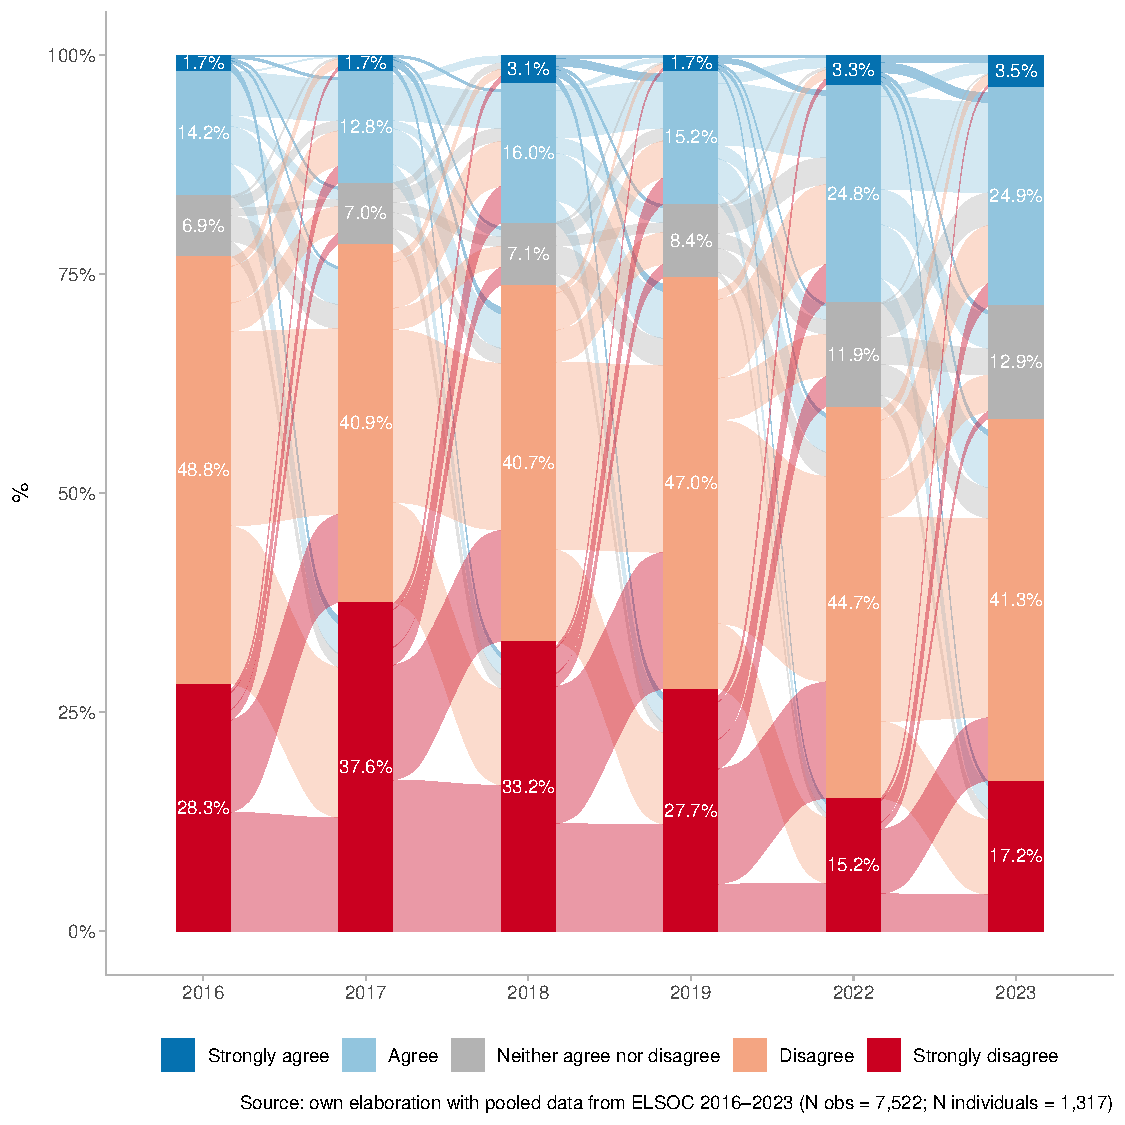
\includegraphics[width=1\linewidth,height=\textheight,keepaspectratio]{paper-blinded_files/figure-pdf/fig-alluvial-1.pdf}

}

\end{figure}%

\subsection{Bivariate relationships}\label{bivariate-relationships}

Figure~\ref{fig-scatter-corr} shows the correlation matrix between
meritocratic perceptions and preferences for pension market justice.
Both effort-based (\(r\) = 0.10, \(p\) \textless{} 0.001) and
talent-based (\(r\) = 0.08, \(p\) \textless{} 0.001) meritocratic
perceptions are positively associated with greater support for
market-based pension welfare. Although these correlations are modest,
their statistical significance indicates a consistent bivariate
relationship. The two meritocracy indicators are also strongly
correlated (\(r\) = 0.68, \(p\) \textless{} 0.001), suggesting they
capture a shared meritocratic worldview while remaining sufficiently
distinct to justify treating them as separate constructs. Taken
together, these patterns provide initial support for the expectation
that meritocratic perceptions are associated with greater acceptance of
income-linked pension outcomes, while also suggesting that other factors
likely account for most of the variation in these preferences.

\begin{figure}[H]

\caption{\label{fig-scatter-corr}Correlation matrix between meritocratic
perceptions and market justice preferences in pension}

\centering{

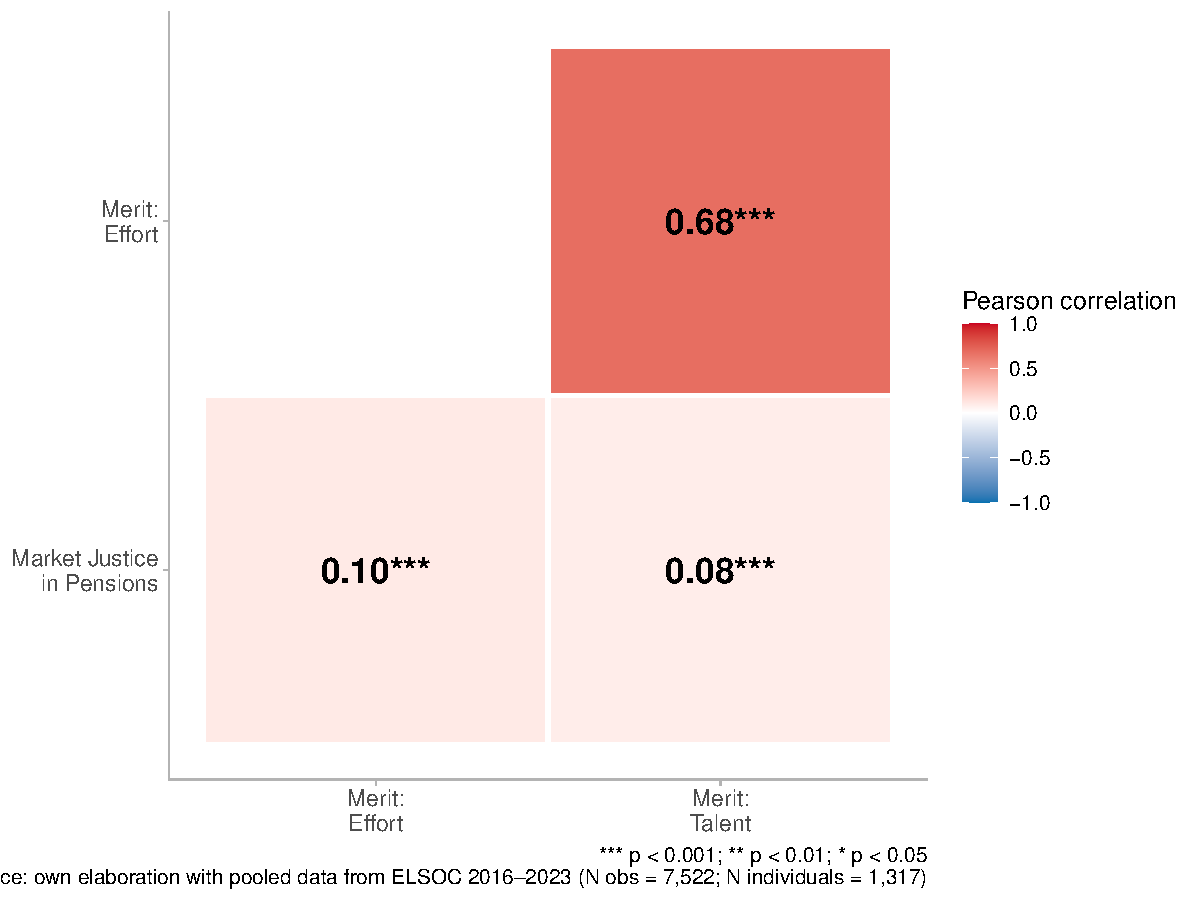
\includegraphics[width=0.85\linewidth,height=\textheight,keepaspectratio]{paper-blinded_files/figure-pdf/fig-scatter-corr-1.pdf}

}

\end{figure}%

Turning to social class differences, Figure~\ref{fig-meanchange} plots
longitudinal trajectories of pension market justice by class from 2016
to 2023. Overall, the descriptive trends suggest that there are no
differences between social classes in their level of preference for
market justice in pensions. The figure shows a broadly upward trend
across all classes, especially after 2019, alongside increasingly
similar levels over time. The unemployed group shows the most
significant change, moving from strong rejection (approximately −0.6 in
2016) to moderate acceptance (approximately 0.7 in 2023).
Retirees/pensioners also increase steadily, from near zero in 2016 to
roughly 0.5 by 2023, and the service class rises notably---particularly
between 2019 and 2022---reaching values close to 0.5. The working class
follows a similar trajectory, though at slightly lower levels. Overall,
the trajectories suggest convergence toward greater acceptance of
pension inequality during 2019--2023, a period marked by social unrest,
the pandemic, and pension fund withdrawals (\emph{10\% retiros}),
raising questions about how these disruptions and the surrounding policy
debate reshaped views of distributive justice.

\begin{figure}[H]

\caption{\label{fig-meanchange}Changes in the standarized mean of market
justice preferences in pensions by social class (2016-2023)}

\centering{

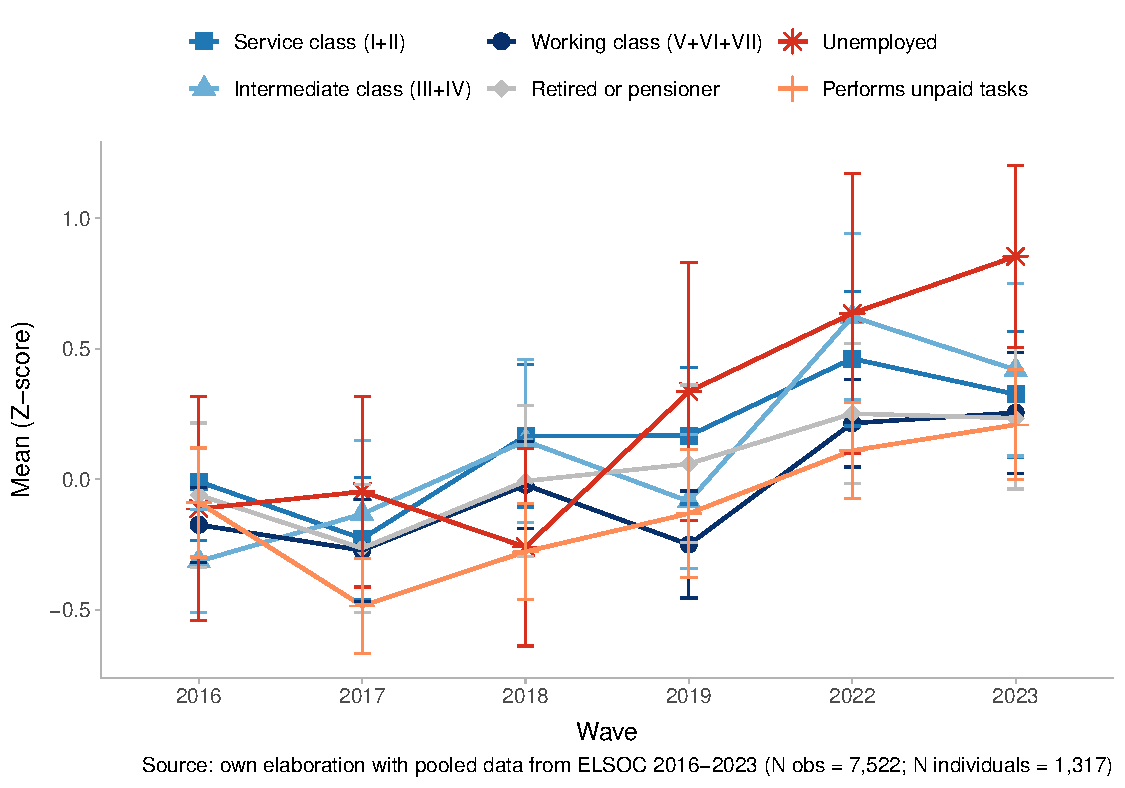
\includegraphics[width=1\linewidth,height=\textheight,keepaspectratio]{paper-blinded_files/figure-pdf/fig-meanchange-1.pdf}

}

\end{figure}%

\subsection{Multilevel models}\label{multilevel-models}

Table~\ref{tbl-modelos} reports estimates from the cumulative
longitudinal multilevel models of support for pension market justice,
distinguishing effects operating between individuals (BE) and within
individuals over time (WE). The intraclass correlation coefficient
(\citeproc{ref-hox_multilevel_2017}{Hox et al., 2017}) from the null
model (see \hyperref[anexo]{Supplementary Material}), which partitions
the total variance in the outcome, is 0.24. This implies that about 24\%
of the variance lies between individuals, while the remaining 76\%
reflects within-person change across survey waves.

\begin{table}

\caption{\label{tbl-modelos}Cumulative link longitudinal multilevel
models for pension market justice preferences}

\centering{

\caption{}
\begin{center}
\scalebox{0.8}{
\begin{tabular}{l c c c c c c}
\hline
 & Model 1 & Model 2 & Model 3 & Model 4 & Model 5 & Model 6 \\
\hline
Wave (Ref.= 2016)                            &                &               &               &               &               &               \\
                                             &                &               &               &               &               &               \\
\quad Wave 2017                              & $-0.337^{***}$ &               &               &               &               &               \\
                                             & $(0.079)$      &               &               &               &               &               \\
\quad Wave 2018                              & $-0.013$       &               &               &               &               &               \\
                                             & $(0.078)$      &               &               &               &               &               \\
\quad Wave 2019                              & $0.086$        &               &               &               &               &               \\
                                             & $(0.077)$      &               &               &               &               &               \\
\quad Wave 2022                              & $0.879^{***}$  &               &               &               &               &               \\
                                             & $(0.078)$      &               &               &               &               &               \\
\quad Wave 2023                              & $0.854^{***}$  &               &               &               &               &               \\
                                             & $(0.077)$      &               &               &               &               &               \\
Wave                                         &                & $-0.182^{**}$ & $-0.179^{**}$ & $-0.187^{**}$ & $-0.190^{**}$ & $-0.192^{**}$ \\
                                             &                & $(0.064)$     & $(0.064)$     & $(0.064)$     & $(0.064)$     & $(0.064)$     \\
Wave$^2$                                     &                & $0.059^{***}$ & $0.058^{***}$ & $0.060^{***}$ & $0.060^{***}$ & $0.060^{***}$ \\
                                             &                & $(0.009)$     & $(0.009)$     & $(0.009)$     & $(0.009)$     & $(0.009)$     \\
Social class (Ref.= Working class (V+VI+VII) &                &               &               &               &               &               \\
                                             &                &               &               &               &               &               \\
\quad Intermediate class (III+IV)            &                &               & $0.096$       & $0.101$       & $0.147$       & $0.185$       \\
                                             &                &               & $(0.120)$     & $(0.121)$     & $(0.118)$     & $(0.117)$     \\
\quad Service class (I+II)                   &                &               & $0.169$       & $0.169$       & $0.158$       & $0.017$       \\
                                             &                &               & $(0.108)$     & $(0.108)$     & $(0.106)$     & $(0.109)$     \\
\quad Retired or pensioner                   &                &               & $0.103$       & $0.096$       & $0.030$       & $0.110$       \\
                                             &                &               & $(0.117)$     & $(0.117)$     & $(0.115)$     & $(0.127)$     \\
\quad Unemployed                             &                &               & $0.101$       & $0.105$       & $0.147$       & $0.119$       \\
                                             &                &               & $(0.158)$     & $(0.158)$     & $(0.155)$     & $(0.152)$     \\
\quad Performs unpaid tasks                  &                &               & $-0.199$      & $-0.198$      & $-0.208$      & $0.029$       \\
                                             &                &               & $(0.110)$     & $(0.111)$     & $(0.109)$     & $(0.113)$     \\
Merit: Effort (WE)                           &                &               &               & $0.114^{**}$  & $0.117^{***}$ & $0.115^{**}$  \\
                                             &                &               &               & $(0.035)$     & $(0.035)$     & $(0.035)$     \\
Merit: Talent (WE)                           &                &               &               & $0.066$       & $0.066$       & $0.067$       \\
                                             &                &               &               & $(0.034)$     & $(0.034)$     & $(0.034)$     \\
Merit: Effort (BE)                           &                &               &               &               & $0.391^{***}$ & $0.387^{***}$ \\
                                             &                &               &               &               & $(0.097)$     & $(0.093)$     \\
Merit: Talent (BE)                           &                &               &               &               & $0.079$       & $0.028$       \\
                                             &                &               &               &               & $(0.097)$     & $(0.094)$     \\
\hline
Controls                                     & No             & No            & No            & No            & No            & Yes           \\
BIC                                          & $19107.264$    & $19166.031$   & $19199.863$   & $19182.632$   & $19144.360$   & $19097.183$   \\
Numb. obs.                                   & $7522$         & $7522$        & $7522$        & $7522$        & $7522$        & $7522$        \\
Num. groups: individuals                     & $1317$         & $1317$        & $1317$        & $1317$        & $1317$        & $1317$        \\
Var: individuals (Intercept)                 & $1.151$        & $1.334$       & $1.302$       & $1.288$       & $1.146$       & $1.014$       \\
Var: individuals, wave                       & $$             & $0.018$       & $0.018$       & $0.015$       & $0.015$       & $0.016$       \\
\hline
\multicolumn{7}{l}{\scriptsize{Note: Cells contain regression coefficients with standard errors in parentheses. $^{***}p<0.001$; $^{**}p<0.01$; $^{*}p<0.05$.}}
\end{tabular}
}
\label{table:coefficients}
\end{center}

}

\end{table}%

Model 1, which adds survey-wave indicators to capture temporal shifts in
the outcome, shows a decline in 2017 (\(\beta\) = -0.337, \(p\)
\textless{} 0.001) relative to 2016. By contrast, the 2022 and 2023
waves exhibit significant increases in market justice preferences for
pension (\(\beta\) = 0.879, \(p\) \textless{} 0.001; \(\beta\) = 0.854,
\(p\) \textless{} 0.001), indicating a nonlinear pattern over time. To
account for this trajectory, Model 2 specifies time (survey wave) as a
continuous predictor and includes a quadratic term to capture the
curvature suggested by Model 1. The negative linear coefficient
indicates an overall downward trend in market-based access to old-age
pension benefits, whereas the positive quadratic term signals a
subsequent upturn in the final measurement points.

Model 3 adds between-group effects (BE) for social class, capturing
differences in average support for pension market justice across class
locations. Overall, the estimates provide no evidence of systematic
class differences in the support for market-based access to old-age
pension benefits. Using the working class as the reference group, those
in the intermediate class (\(\beta\) = 0.10, \(p\) \textgreater{} 0.05),
the service class (\(\beta\) = 0.17, \(p\) \textgreater{} 0.05),
retirees (\(\beta\) = 0.10, \(p\) \textgreater{} 0.05), and the
unemployed (\(\beta\) = 0.10, \(p\) \textgreater{} 0.05) exhibit
positive coefficients, but none reach conventional levels of statistical
significance. Likewise, individuals performing unpaid work (e.g.,
domestic or care work) show a negative coefficient relative to the
working class, which is not statistically significant (\(\beta\) =
-0.20, \(p\) \textgreater{} 0.05). Taken together, these results suggest
that neither class position nor being outside the labour force is
clearly associated with differences in preferences for pension market
justice at the between-individual level.

Models 4 and 5 extend the analysis by incorporating the within-person
(WE) and between-person (BE) components of the meritocratic variables.
Model 4 examines how changes in individuals' meritocratic perceptions
over time relate to their views on pension market justice. The estimates
show that the within-effect of perceiving that effort is rewarded is
positive and highly significant (\(p\) \textless{} 0.001). Holding all
other predictors constant, a one-point increase in effort-based
meritocratic perceptions for the same respondent between waves is
associated with a 0.11-point increase in the support for market-based
access to old-age pension benefits. Model 5, which captures
between-person differences, points in the same direction. On average,
respondents who see their society as more effort-meritocratic display
stronger market-oriented views on pensions, with a 0.39-point higher
score on the outcome, a statistically significant association. By
contrast, the corresponding indicators for the perception that
intelligence and ability are rewarded show no statistically significant
association with the support for pension market justice at either the
within (\(\beta\) = 0.07, \(p\) \textgreater{} 0.05)- or between-person
level (\(\beta\) = 0.08, \(p\) \textgreater{} 0.05).

\begin{figure}[H]

\caption{\label{fig-interaction1}Predicted probabilities of pension
market justice preferences by talent-based meritocratic perceptions and
social class}

\centering{

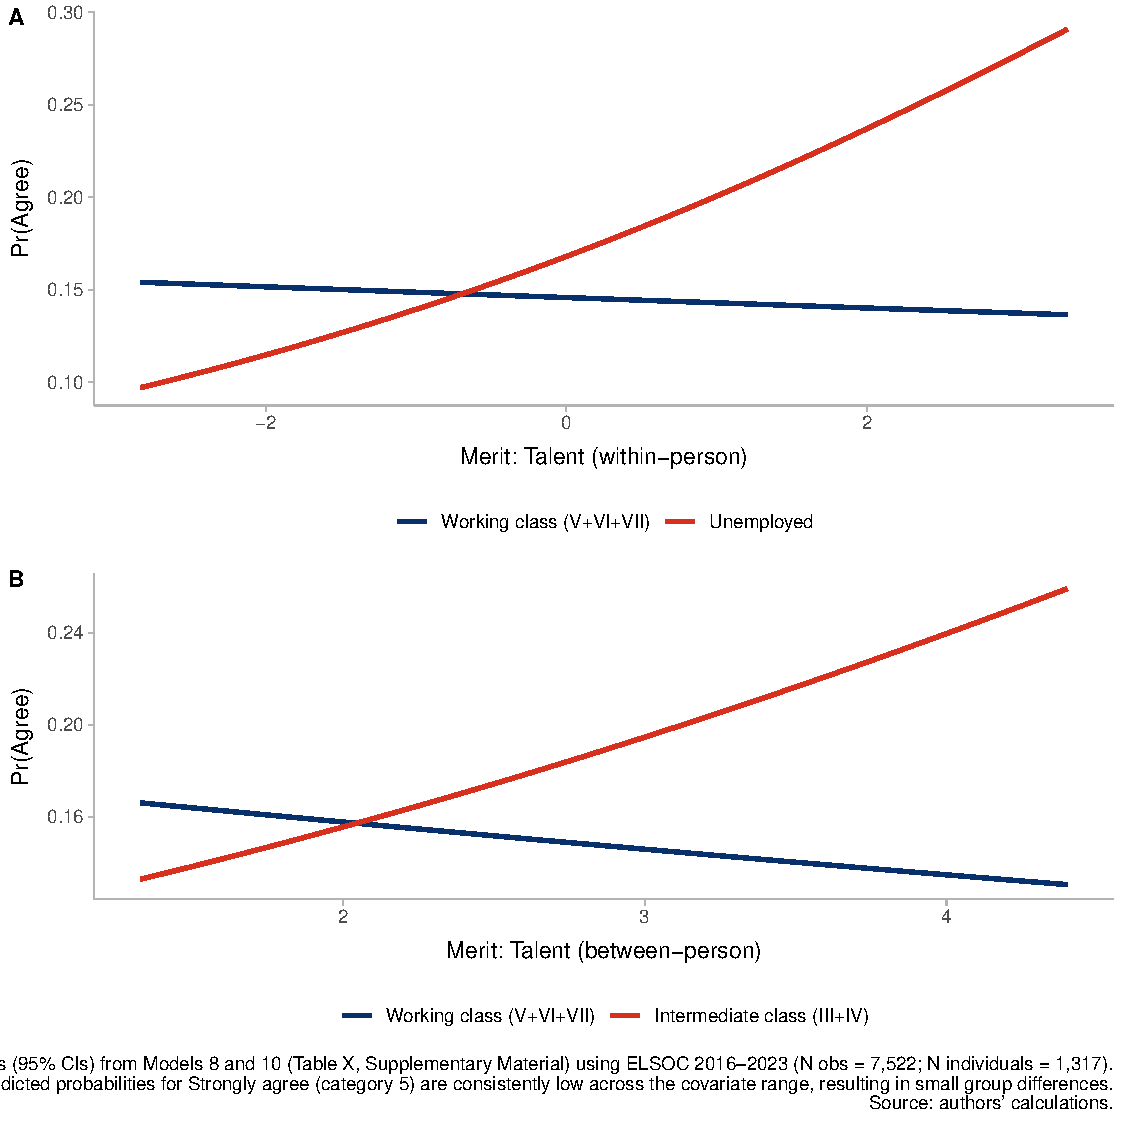
\includegraphics[width=0.8\linewidth,height=\textheight,keepaspectratio]{paper-blinded_files/figure-pdf/fig-interaction1-1.pdf}

}

\end{figure}%

Model 6 introduces the control variables. The within- and
between-effects of the main predictors remain stable in both sign and
significance, indicating that the associations are robust (see
\hyperref[anexo]{Supplementary Material} for the effects of the control
variables).

To examine whether meritocratic perceptions condition class differences
in pension market justice preferences, we estimate four interaction
models that combine between-person social class with the within- and
between-person components of meritocratic perceptions. Overall,
interaction terms are small and generally not statistically
distinguishable from zero, and improvements in model fit over the
baseline specifications are modest. This pattern indicates that the
association between meritocratic perceptions and support for
market-based pension allocation is similar across class locations
(complete model estimates are reported in the
\hyperref[anexo]{Supplementary Material}).

Two interaction effects nevertheless stand out, which are illustrated in
Figure~\ref{fig-interaction1}. First, panel A shows that the
within-person association between talent-based meritocratic perceptions
and pension market justice differs by labour-market status.
Within-person deviations in perceived talent rewards are unrelated to
pension market justice in the reference group (\(\beta\) = −0.024, \(p\)
= .67), but become significantly more positive among unemployed
respondents (interaction \(\beta\) = 0.257, \(p\) = .049), implying a
net within-person effect of \(\beta\) = 0.233 (OR ≈ 1.26). Second, panel
B indicates that the between-person association between average
(person-mean) talent-based meritocratic perceptions and pension market
justice varies by social class: it is null in the working class
(\(\beta\) = −0.089, \(p\) = .50) but significantly stronger in the
intermediate class (interaction \(\beta\) = 0.401, \(p\) = .035),
yielding a positive between-person slope of \(\beta\) = 0.313 (OR ≈
1.37). Taken together, these models indicate a largely homogeneous
association between meritocratic beliefs and pension market justice,
with limited evidence of moderation. Where moderation emerges, it is
concentrated in the talent dimension and confined to specific
middle-class and non-class positions rather than reflecting systematic
stratification across the whole class structure.

\section{Discussion}\label{discussion}

Regarding descriptive trends, survey data from 2016 to 2023 reveal a
persistent tension in Chileans' judgments regarding pension market
justice. In every wave, clear majorities reject the idea that it is fair
for higher-income individuals to receive better pensions than
lower-income individuals. At the same time, a small---but
expanding---segment endorses this income-based principle, with the
sharpest growth occurring between 2018 and 2023. Pension market justice,
therefore, remains a minority orientation, yet one that has become more
prevalent over time, in line with longitudinal evidence of rising
support for income-based access to other welfare services in Chile, such
as healthcare and education
(\citeproc{ref-castillo_perceptions_2025}{Castillo et al., 2025}). These
attitudes are formed within an institutional architecture of mandatory,
privately managed, defined-contribution accounts that tightly link
old-age income to labor earnings, contribution stability, and market
performance (\citeproc{ref-madero-cabib_private_2019}{Madero-Cabib et
al., 2019}; \citeproc{ref-solimano_rise_2021}{Solimano, 2021}), and that
can symbolically recast pensions from solidarity-based social rights
into individual financial assets. In this respect, Chile mirrors broader
findings that income-based access to welfare is more strongly endorsed
in liberal, marketised regimes (\citeproc{ref-lindh_public_2015}{Lindh,
2015}). Taken together, these descriptive patterns suggest that support
for pension market justice---contested and far from
hegemonic---nonetheless constitutes a salient orientation that invites
explanation: which social trajectories and belief structures sustain it?

Concerning social class, the results provide no support for \(H_1\),
which predicted stronger endorsement of pension market justice among the
upper classes than among the lower classes. The longitudinal multilevel
models indicate that neither the intermediate class nor the service
class differs significantly from the working class in their pension
market justice preferences. This null finding is substantively
meaningful because it indicates that class position---despite being a
fundamental structural determinant of pension outcomes in Chile's
individual capitalization system
(\citeproc{ref-galvez_pensiones_2024}{Gálvez et al., 2024};
\citeproc{ref-madero-cabib_private_2019}{Madero-Cabib et al.,
2019})---does not translate into systematic differences in attitudes
toward the system's distributive logic. Moreover, the lack of
significant class effects persists across most specifications,
suggesting that this is a robust empirical pattern rather than an
artifact of a particular model choice or set of controls.

This absence of class differentiation contradicts expectations derived
from material interests (\citeproc{ref-lindh_public_2015}{Lindh, 2015};
\citeproc{ref-svallfors_moral_2006}{Svallfors, 2006}) and contrasts with
evidence from developed welfare states
(\citeproc{ref-busemeyer_welfare_2020}{Busemeyer \& Iversen, 2020};
\citeproc{ref-lindh_public_2015}{Lindh, 2015}) and from market-oriented
welfare configurations in Latin America
(\citeproc{ref-kerner_pension_2020}{Kerner, 2020}), where privileged
groups tend to endorse market allocation more strongly than lower
classes. The result is particularly striking given the system's sharply
unequal material consequences across class positions: while privileged
groups with stable formal employment can secure higher pensions through
sustained contributions, working-class trajectories are more often
precarious and yield insufficient retirement income
(\citeproc{ref-cabib_avoiding_2025}{Cabib, 2025};
\citeproc{ref-gil-hernandez_wealth_2025}{Gil-Hernández et al., 2025}). A
plausible interpretation of this disconnection between objective class
interests and subjective justice evaluations lies in the individualising
logic of Chile's capitalization system, which reframes distributive
conflict away from class-based struggles and toward individualized
responsibility (\citeproc{ref-arrizabalomontoro_debate_2019}{Arrizabalo
Montoro et al., 2019}). By presenting pensions as the direct outcome of
personal contributions and choices, the system may obscure the extent to
which ``contributory capacity'' itself reflects structural inequalities
rather than individual merit, thereby weakening the attitudinal imprint
of class position---even among those most disadvantaged by the market
model.

This phenomenon of ``class neutralization'' contrasts sharply with the
established findings of comparative research on welfare, in which class
position tends to shape distributive preferences in predictable ways
(\citeproc{ref-svallfors_moral_2006}{Svallfors, 2006};
\citeproc{ref-svallfors_political_2007}{Svallfors, 2007}). While
previous studies in both developed welfare states
(\citeproc{ref-busemeyer_welfare_2020}{Busemeyer \& Iversen, 2020};
\citeproc{ref-lindh_public_2015}{Lindh, 2015}) and in Latin American
contexts (\citeproc{ref-kerner_pension_2020}{Kerner, 2020}) document
more market-oriented attitudes among privileged groups, our results
suggest that decades of pension privatization may have eroded this
class-based differentiation by incorporating individualized
responsibility as the dominant normative framework.

Turning to meritocratic perceptions, \(H_{2a}\) and \(H_{2b}\) predicted
that stronger meritocratic perceptions would be associated with greater
support for market-based access to pensions. The results offer partial
but revealing support for this hypothesis. At the between-person level
(BE), the perception that effort is rewarded in society is strongly
positively associated with pension market justice. In contrast, the
perception that talent is rewarded is not statistically significant. At
the within-person level (WE), effort-based meritocratic perceptions also
show a significant positive association, albeit of smaller magnitude,
whereas talent remains non-significant. Substantively, this means that
individuals who, on average, perceive more substantial effort--reward
linkages are more supportive of pension market justice, and individuals
who increase their effort-based meritocratic perceptions over time also
tend to increase their support for pension market justice. The contrast
between effort and talent suggests that when people justify pension
market allocation, they draw primarily on narratives of hard work and
responsibility rather than on innate ability.

These findings align with a broader view of meritocracy as a
legitimising ideology in highly unequal contexts. In Chile's individual
capitalization system, where pensions are institutionally presented as
the direct result of personal contributions and choices, the effort
narrative provides a compelling cognitive frame for justifying
disparities: higher pensions can be interpreted as the deserved outcome
of ``working harder,'' regardless of the structural constraints faced by
different groups (\citeproc{ref-castillo_perceptions_2025}{Castillo et
al., 2025}). This pattern echoes scholarship suggesting that
meritocratic perceptions can intensify precisely where real
opportunities are most constrained
(\citeproc{ref-harrs_fairness_2025}{Harrs \& Sterba, 2025};
\citeproc{ref-mijs_paradox_2021}{Mijs, 2021}). Importantly, the
explanatory power of effort-based perceptions also helps contextualise
the null class pattern observed for \(H_1\): meritocratic ideology can
offer a culturally available justification that renders unequal pension
outcomes intelligible and acceptable, thereby dampening the extent to
which class position translates into divergent justice evaluations.

Against this backdrop, a primary interest of the study was to examine
whether meritocratic perceptions condition class differences in pension
market justice (\(H_{3a}\) and \(H_{3b}\)), with more substantial
meritocratic effects expected among higher classes. The results point to
a more selective and class-specific pattern than initially hypothesised.
Rather than a generalized moderation among the service class,
meritocratic perceptions---particularly talent-based ones---operate
primarily among the intermediate class. At the between-person level
(\(H_{3a}\)), this class exhibits a significant positive interaction
with talent-based meritocratic perceptions, indicating that
intermediate-class individuals who hold stronger and more stable beliefs
that talent is rewarded are more likely to support pension
commodification. In contrast, no comparable interaction emerges for
effort, and no equivalent moderation appears within the service class.
One interpretation is that those in the most advantaged positions may
have less need to rely on talent-based justifications because their
outcomes can be plausibly narrated through dominant accounts of
sustained effort, credentials, and accumulated advantages
(\citeproc{ref-lindh_class_2020}{Lindh \& McCall, 2020}). The
within-person analysis (\(H_{3b}\)) further qualifies the moderation
story: intra-individual changes in meritocratic perceptions do not
generally moderate the relationship between class and pension market
justice for either effort or talent, suggesting that short-term
fluctuations are insufficient to reshape class-linked orientations and
that what matters more are stable, long-term orientations---particularly
toward talent as a distributive principle---within specific class
locations.

An important exception, however, emerges for unemployed respondents.
Within-person deviations in perceived talent rewards are unrelated to
pension market justice in the working class, but become significantly
more positive among the unemployed. Substantively, this indicates that
among unemployed individuals, increases over time in the perception that
talent is rewarded are associated with higher support for pension market
justice. A posible interpretation of this caveat is that unemployment
weakens the experiential plausibility of effort-based narratives. When
one's effort is not being translated into employment or stable
contributions, talent may become a more salient explanatory lens for
unequal outcomes in core welfare domains such as pensions. In this
sense, the unemployed may be especially prone to shifting toward
talent-based meritocratic accounts to explain distributive differences,
and these shifts, in turn, are associated with greater endorsement of
market-based pension justice.

Taken together, these findings suggest that in a context where effort
does not reliably translate into secure welfare outcomes---such as
Chile's privatized, individual-contribution pension system---the
intermediate class may more readily draw on talent-based explanations to
legitimise modest relative advantages and to rationalise why increased
effort does not necessarily yield service-class outcomes
(\citeproc{ref-castillo_perceptions_2025}{Castillo et al., 2025};
\citeproc{ref-lindh_class_2020}{Lindh \& McCall, 2020}). The service
class, by contrast, appears less dependent on this symbolic
reinforcement, as its privileged position can be more coherently
explained through widely shared narratives of effort and qualifications.

\section{Conclusion}\label{conclusion}

This article examined the complex interaction between social class,
meritocratic perceptions, and preferences for market justice in the
Chilean pension system during the period between 2016 and 2023. Using
longitudinal data from the ELSOC survey, we explored how the individual
capitalization model---a system that links old-age benefits to personal
contributions---shapes the normative foundations of social justice. By
analyzing these dynamics during a period marked by significant social
unrest and political discussions around a new constitution, the study
offers a critical view of how market logic and subjective beliefs about
equity coexist in a highly unequal and commodified environment.

The findings reveal a paradox where objective social class does not
significantly predict attitudes toward pension market justice; instead,
support for income-based pension differences grew across all strata,
reaching nearly 28.4\% by 2023. This suggests that the individualizing
logic of the pension system has succeeded in reframing distributive
conflicts as matters of personal responsibility, leading to a
generalised pattern of beliefs across classes and supporting the idea of
markets as moral projects (\citeproc{ref-fourcade_moral_2007}{Fourcade
\& Healy, 2007}). Meritocratic perceptions, specifically those
emphasizing individual effort, were found to be the primary drivers of
this support, acting as a powerful moral justification that allows
individuals to legitimize pension disparities regardless of their own
structural disadvantages. While effort-based beliefs remained stable
predictors of fairness, talent-based justifications emerged more
selectively, particularly within the intermediate class, as a tool to
rationalize modest relative advantages.

This research advances on previous work by shifting the focus from
objective socio-economic measures to the longitudinal, subjective
interplay of class and meritocratic ideology. Unlike previous studies
that assume material interests automatically dictate policy preferences,
this work emphasizes how a ``policy feedback'' mechanism in a privatized
regime can erode class-based demands for redistribution. The study
underscores how the Chilean model symbolically recasts social rights as
financial assets, illustrating the resilience of meritocratic narratives
even in the face of widespread public discontent and systemic
inequality.

In terms of pathways for future research, international comparative
studies are needed to determine whether this `class neutralization' is
unique to Chile's neoliberal history or whether it is a universal
feature of privatized welfare regimes. Future studies should also
explore the role of political communication, and discussions on pensions
funds withdrawals during the pandemic, on changing perceptions of
pension ownership and fairness. Also, investigating how these normative
beliefs translate into behavioral -- as voting patterns or participation
in social movements such as `No+AFP' --- would provide valuable insights
into the path from subjective perceptions to actual policy change.
Finally, it is also important to consider how to integrate new measures
of meritocracy (\citeproc{ref-castillo_multidimensional_2023}{Castillo
et al., 2023}) into future studies, as this could reveal other
configurations of beliefs between preferences for market justice and
merit that the current operationalization does not allow to observe.

\section{References}\label{references}

\phantomsection\label{refs}
\begin{CSLReferences}{1}{0}
\bibitem[\citeproctext]{ref-alesina_fairness_2005}
Alesina, A., \& Angeletos, G. (2005). Fairness and redistribution.
\emph{American Economic Review}, 960--980.

\bibitem[\citeproctext]{ref-alesina_preferences_2005}
Alesina, Alberto, \& La Ferrara, E. (2005). Preferences for
redistribution in the land of opportunities. \emph{Journal of Public
Economics}, \emph{89}(5-6), 897--931.
\url{https://doi.org/10.1016/j.jpubeco.2004.05.009}

\bibitem[\citeproctext]{ref-arenas_sistemas_2019}
Arenas, A. (2019). \emph{Los sistemas de pensiones en la encrucijada:
desafíos para la sostenibilidad en América Latina}. Santiago: Naciones
Unidas, CEPAL.

\bibitem[\citeproctext]{ref-arrizabalomontoro_debate_2019}
Arrizabalo Montoro, X., Del Rosal, M., \& Javier Murillo Arroyo, F.
(2019). The debate on pension systems: The paradigmatic cases of chile
and spain. \emph{The American Journal of Economics and Sociology},
\emph{78}(1), 195--223. \url{https://doi.org/10.1111/ajes.12262}

\bibitem[\citeproctext]{ref-barone_rise_2022}
Barone, C., Hertel, F. R., \& Smallenbroek, O. (2022). The rise of
income and the demise of class and social status? A systematic review of
measures of socio-economic position in stratification research.
\emph{Research in Social Stratification and Mobility}, \emph{78},
100678. \url{https://doi.org/10.1016/j.rssm.2022.100678}

\bibitem[\citeproctext]{ref-barozet_measurement_2021}
Barozet, E., Boado, M., \& Marqués-Perales, I. (2021). The measurement
of social stratification: Comparative perspectives between europe and
latin america. In P. López-Roldán \& S. Fachelli (Eds.), \emph{Towards a
comparative analysis of social inequalities between europe and latin
america} (pp. 171--202). Cham: Springer International Publishing.
\url{https://doi.org/10.1007/978-3-030-48442-2_6}

\bibitem[\citeproctext]{ref-barriga_pensiones_2024}
Barriga, F., \& Kremerman, M. (2024). Pensiones sin Seguridad Social:
¿Cómo se calcula el monto de las pensiones en Chile? \emph{Fundación
Sol}.

\bibitem[\citeproctext]{ref-beland_varieties_2019}
Béland, D., \& Schlager, E. (2019). Varieties of policy feedback
research: Looking backward, moving forward. \emph{Policy Studies
Journal}, \emph{47}(2), 184--205.
\url{https://doi.org/10.1111/psj.12340}

\bibitem[\citeproctext]{ref-bell_fixed_2019}
Bell, A., Fairbrother, M., \& Jones, K. (2019). Fixed and random effects
models: Making an informed choice. \emph{Quality \& Quantity},
\emph{53}(2), 1051--1074.
\url{https://doi.org/10.1007/s11135-018-0802-x}

\bibitem[\citeproctext]{ref-bell_explaining_2015}
Bell, A., \& Jones, K. (2015). Explaining fixed effects: Random effects
modeling of time-series cross-sectional and panel data. \emph{Political
Science Research and Methods}, \emph{3}(1), 133--153.
\url{https://doi.org/10.1017/psrm.2014.7}

\bibitem[\citeproctext]{ref-boccardo_30_2020}
Boccardo, G. (2020). \emph{30 años de privatizaciones en chile: Lo que
la pandemia reveló}. Nodo XXI.

\bibitem[\citeproctext]{ref-borzutzky_chiles_2016}
Borzutzky, S., \& Hyde, M. (2016). Chile's private pension system at 35:
Impact and lessons. \emph{Journal of International and Comparative
Social Policy}, \emph{32}(1), 57--73.
\url{https://doi.org/10.1080/21699763.2016.1148623}

\bibitem[\citeproctext]{ref-bottero_class_2004}
Bottero, W. (2004). Class identities and the identity of class.
\emph{Sociology}, \emph{38}(5), 985--1003.
\url{https://doi.org/10.1177/0038038504047182}

\bibitem[\citeproctext]{ref-breznau_institutional_2023}
Breznau, N. (2023). Institutional trajectories of the welfare state:
Returns from social policy inception to modern public opinion. In F.
Roosma \& T. Laenen (Eds.), \emph{A research agenda for public attitudes
to welfare} (pp. 185--205). Edward Elgar Publishing.
\url{https://doi.org/10.4337/9781800887411.00015}

\bibitem[\citeproctext]{ref-busemeyer_education_2013}
Busemeyer, M. R. (2013). Education funding and individual preferences
for redistribution. \emph{European Sociological Review}, \emph{29}(6),
1122--1133. \url{https://doi.org/10.1093/esr/jcs085}

\bibitem[\citeproctext]{ref-busemeyer_skills_2015}
Busemeyer, M. R. (2015). \emph{Skills and inequality: Partisan politics
and the political economy of education reforms in western welfare
states}. Cambridge: Cambridge University Press.
\url{https://doi.org/10.1017/CBO9781107477650}

\bibitem[\citeproctext]{ref-busemeyer_welfare_2020}
Busemeyer, M. R., \& Iversen, T. (2020). The welfare state with private
alternatives: The transformation of popular support for social
insurance. \emph{The Journal of Politics}, \emph{82}(2), 671--686.
\url{https://doi.org/10.1086/706980}

\bibitem[\citeproctext]{ref-cabib_avoiding_2025}
Cabib, I. (2025). \emph{Avoiding retirement in chile: Extending working
lives in an uncertain and precarious context}. London: Routledge.

\bibitem[\citeproctext]{ref-canalesceron_sujeto_2021}
Canales Cerón, M., Orellana Calderón, V. S., \& Guajardo Mañán, F.
(2021). Sujeto y cotidiano en la era neoliberal: El caso de la educación
chilena. \emph{Revista Mexicana de Ciencias Políticas y Sociales},
\emph{67}(244).
\url{https://doi.org/10.22201/fcpys.2448492xe.2022.244.70386}

\bibitem[\citeproctext]{ref-castillo_multidimensional_2023}
Castillo, J. C., Iturra, J., Maldonado, L., Atria, J., \& Meneses, F.
(2023). A multidimensional approach for measuring meritocratic beliefs:
Advantages, limitations and alternatives to the ISSP social inequality
survey. \emph{International Journal of Sociology}, \emph{53}(6),
448--472. \url{https://doi.org/10.1080/00207659.2023.2274712}

\bibitem[\citeproctext]{ref-castillo_perceptions_2025}
Castillo, J. C., Laffert, A., Carrasco, K., \& Iturra-Sanhueza, J.
(2025). Perceptions of inequality and meritocracy: Their interplay in
shaping preferences for market justice in chile (2016--2023).
\emph{Frontiers in Sociology}, \emph{10}, 1634219.
\url{https://doi.org/10.3389/fsoc.2025.1634219}

\bibitem[\citeproctext]{ref-castillo_deserving_2019}
Castillo, J. C., Olivos, F., \& Azar, A. (2019). Deserving a just
pension: A factorial survey approach*. \emph{Social Science Quarterly},
\emph{100}(1), 359--378. \url{https://doi.org/10.1111/ssqu.12539}

\bibitem[\citeproctext]{ref-castillo_socialization_2024}
Castillo, J. C., Salgado, M., Carrasco, K., \& Laffert, A. (2024). The
socialization of meritocracy and market justice preferences at school.
\emph{Societies}, \emph{14}(11), 214.
\url{https://doi.org/10.3390/soc14110214}

\bibitem[\citeproctext]{ref-chancel_world_2025}
Chancel, L., Gómez-Carrera, R., Moshrif, R., \& Piketty, T. (2025).
World inequality report 2026. \emph{World Inequality Lab},
\emph{wir2026.wid.world}.

\bibitem[\citeproctext]{ref-dodson_economic_2017}
Dodson, K. (2017). Economic change and class conflict over tax
attitudes: Evidence from nine advanced capitalist democracies.
\emph{Social Forces}, \emph{95}(4), 1509--1538.
\url{https://doi.org/10.1093/sf/sox027}

\bibitem[\citeproctext]{ref-erikson_constant_1992}
Erikson, R., \& Goldthorpe, J. (1992a). \emph{The constant flux: A study
of class mobility in industrial societies}. Oxford: Clarendon Pr.

\bibitem[\citeproctext]{ref-erikson_casmin_1992}
Erikson, R., \& Goldthorpe, J. H. (1992b). The CASMIN project and the
american dream. \emph{European Sociological Review}, \emph{8}(3),
283--305. \url{https://doi.org/10.1093/oxfordjournals.esr.a036642}

\bibitem[\citeproctext]{ref-esping-andersen_three_1990}
Esping-Andersen, G. (1990). \emph{The three worlds of welfare
capitalism}. Cambridge: Polity Press.

\bibitem[\citeproctext]{ref-ferre_welfare_2023}
Ferre, J. C. (2023). Welfare regimes in twenty-first-century latin
america. \emph{Journal of International and Comparative Social Policy},
\emph{39}(2), 101--127. \url{https://doi.org/10.1017/ics.2023.16}

\bibitem[\citeproctext]{ref-ffrench-davis_reformas_2018}
Ffrench-Davis, R. (2018). \emph{Reformas económicas en Chile 1973-2017}.
TAURUS.

\bibitem[\citeproctext]{ref-flores_top_2020}
Flores, I., Sanhueza, C., Atria, J., \& Mayer, R. (2020). Top incomes in
chile: A historical perspective on income inequality, 1964--2017.
\emph{Review of Income and Wealth}, \emph{66}(4), 850--874.
\url{https://doi.org/10.1111/roiw.12441}

\bibitem[\citeproctext]{ref-fourcade_moral_2007}
Fourcade, M., \& Healy, K. (2007). Moral views of market society.
\emph{Annual Review of Sociology}, \emph{33}(Volume 33, 2007), 285--311.
\url{https://doi.org/10.1146/annurev.soc.33.040406.131642}

\bibitem[\citeproctext]{ref-galvez_pensiones_2024}
Gálvez, R., Kremerman, M., \& Palacios, V. R. (2024). Pensiones bajo el
mínimo: Los montos de las pensiones que paga el sistema de
capitalización individual en Chile. \emph{Fundación Sol}.

\bibitem[\citeproctext]{ref-gil-hernandez_wealth_2025}
Gil-Hernández, C. J., Salas-Rojo, P., Vidal, G., \& Villani, D. (2025).
Wealth and income stratification by social class in five european
countries. \emph{Social Indicators Research}, \emph{178}(2), 817--841.
\url{https://doi.org/10.1007/s11205-025-03532-x}

\bibitem[\citeproctext]{ref-harrs_fairness_2025}
Harrs, S., \& Sterba, M.-B. (2025). \emph{Fairness and support for
redistribution: The role of preferences and beliefs}. University of
Konstanz. \url{https://doi.org/10.48787/KOPS/352-2-1795HQRPSTDTX1}

\bibitem[\citeproctext]{ref-haubo_cumulative_2018}
Haubo, R., \& Christensen, B. (2018). Cumulative link models for ordinal
regression with the r package ordinal. In.

\bibitem[\citeproctext]{ref-hox_multilevel_2017}
Hox, J., Moerbeek, M., \& Schoot, R. van de. (2017). \emph{Multilevel
analysis: Techniques and applications, third edition} (3rd ed.). New
York: Routledge. \url{https://doi.org/10.4324/9781315650982}

\bibitem[\citeproctext]{ref-huber_political_2000}
Huber, E., \& Stephens, J. D. (2000). The political economy of pension
reform: Latin america in comparative perspective. \emph{Occasional
Paper}, (7).

\bibitem[\citeproctext]{ref-hyde_chiles_2015}
Hyde, M., \& Borzutzky, S. (2015). Chile's {``neoliberal''} retirement
system? Concentration, competition, and economic predation in
{``private''} pensions: Chile's {``neoliberal''} retirement system?
\emph{Poverty \& Public Policy}, \emph{7}(2), 123--157.
\url{https://doi.org/10.1002/pop4.98}

\bibitem[\citeproctext]{ref-immergut_it_2020}
Immergut, E. M., \& Schneider, S. M. (2020). Is it unfair for the
affluent to be able to purchase {``better''} healthcare? Existential
standards and institutional norms in healthcare attitudes across 28
countries. \emph{Social Science \& Medicine}, \emph{267}, 113146.
\url{https://doi.org/10.1016/j.socscimed.2020.113146}

\bibitem[\citeproctext]{ref-jaime-castillo_public_2013}
Jaime-Castillo, A. M. (2013). Public opinion and the reform of the
pension systems in europe: The influence of solidarity principles.
\emph{Journal of European Social Policy}, \emph{23}(4), 390--405.
\url{https://doi.org/10.1177/0958928713507468}

\bibitem[\citeproctext]{ref-kerner_pension_2020}
Kerner, A. (2020). Pension returns and popular support for neoliberalism
in post-pension reform latin america. \emph{British Journal of Political
Science}, \emph{50}(2), 585--620.
\url{https://doi.org/10.1017/S0007123417000710}

\bibitem[\citeproctext]{ref-kluegel_legitimation_1999}
Kluegel, J., Mason, D., \& Wegener, B. (1999). The legitimation of
capitalism in the postcommunist transition: Public opinion about market
justice, 1991-1996. \emph{European Sociological Review}, \emph{15}(3),
33. Retrieved from \url{https://www.jstor.org/stable/522731}

\bibitem[\citeproctext]{ref-kluegel_beliefs_1981}
Kluegel, J., \& Smith, E. (1981). Beliefs about stratification.
\emph{Annual Review of Sociology}, \emph{7}(Volume 7, 1981), 29--56.
\url{https://doi.org/10.1146/annurev.so.07.080181.000333}

\bibitem[\citeproctext]{ref-koos_moral_2019}
Koos, S., \& Sachweh, P. (2019). The moral economies of market
societies: Popular attitudes towards market competition, redistribution
and reciprocity in comparative perspective. \emph{Socio-Economic
Review}, \emph{17}(4), 793--821.
\url{https://doi.org/10.1093/ser/mwx045}

\bibitem[\citeproctext]{ref-korpi_power_2006}
Korpi, W. (2006). Power resources and employer-centered approaches in
explanations of welfare states and varieties of capitalism:
Protagonists, consenters, and antagonists. \emph{World Politics},
\emph{58}(2), 167--206. \url{https://doi.org/10.1353/wp.2006.0026}

\bibitem[\citeproctext]{ref-korpi_democratic_2018}
Korpi, W. (2018). \emph{The democratic class struggle} (1st ed.).
Routledge. \url{https://doi.org/10.4324/9780429441714}

\bibitem[\citeproctext]{ref-korpi_new_2003}
Korpi, W., \& Palme, J. (2003). New politics and class politics in the
context of austerity and globalization: Welfare state regress in 18
countries, 1975--95. \emph{American Political Science Review},
\emph{97}(03). \url{https://doi.org/10.1017/S0003055403000789}

\bibitem[\citeproctext]{ref-kulin_class_2013}
Kulin, J., \& Svallfors, S. (2013). Class, values, and attitudes towards
redistribution: A european comparison. \emph{European Sociological
Review}, \emph{29}(2), 155--167.
\url{https://doi.org/10.1093/esr/jcr046}

\bibitem[\citeproctext]{ref-lane_market_1986}
Lane, R. E. (1986). Market justice, political justice. \emph{American
Political Science Review}, \emph{80}(2), 383--402.
\url{https://doi.org/10.2307/1958264}

\bibitem[\citeproctext]{ref-langsaether_more_2020}
Langsæther, P. E., \& Evans, G. (2020). More than self‐interest: Why
different classes have different attitudes to income inequality.
\emph{The British Journal of Sociology}, \emph{71}(4), 594--607.
\url{https://doi.org/10.1111/1468-4446.12747}

\bibitem[\citeproctext]{ref-langsaether_explaining_2022}
Langsæther, P. E., Evans, G., \& O'Grady, T. (2022). Explaining the
relationship between class position and political preferences: A
long-term panel analysis of intra-generational class mobility.
\emph{British Journal of Political Science}, \emph{52}(2), 958--967.
\url{https://doi.org/10.1017/S0007123420000599}

\bibitem[\citeproctext]{ref-lee_fairness_2024}
Lee, J.-S., \& Stacey, M. (2024). Fairness perceptions of educational
inequality: The effects of self-interest and neoliberal orientations.
\emph{The Australian Educational Researcher}, \emph{51}(4), 1215--1237.
\url{https://doi.org/10.1007/s13384-023-00636-6}

\bibitem[\citeproctext]{ref-liebig_sociology_2016}
Liebig, S., \& Sauer, C. (2016). Sociology of justice. In C. Sabbagh \&
M. Schmitt (Eds.), \emph{Handbook of social justice theory and research}
(pp. 37--59). New York: Springer.
\url{https://doi.org/10.1007/978-1-4939-3216-0_3}

\bibitem[\citeproctext]{ref-lindh_public_2015}
Lindh, A. (2015). Public opinion against markets? Attitudes towards
market distribution of social services -- a comparison of 17 countries.
\emph{Social Policy \& Administration}, \emph{49}(7), 887--910.
\url{https://doi.org/10.1111/spol.12105}

\bibitem[\citeproctext]{ref-lindh_it_2017}
Lindh, A. (2017). Is it just that people with higher incomes can buy
better education and health care? \emph{57225}, \emph{17}, 69--80.

\bibitem[\citeproctext]{ref-lindh_class_2020}
Lindh, A., \& McCall, L. (2020). Class position and political opinion in
rich democracies. \emph{Annual Review of Sociology}, \emph{46}(1),
419--441. \url{https://doi.org/10.1146/annurev-soc-121919-054609}

\bibitem[\citeproctext]{ref-littler_meritocracy_2018}
Littler, J. (2018). \emph{Against meritocracy: Culture, power and myths
of mobility}. Abingdon, Oxon New York, NY: Routledge, an imprint of the
Taylor \& Francis group.

\bibitem[\citeproctext]{ref-llambias-wolff_political_2019}
Llambías-Wolff, J. (2019). The political economy of health reforms in
chile: A case study of the privatization process. In D. Burke, P.
Godbole, \& A. Cash (Eds.), \emph{Hospital transformation} (pp. 59--70).
Cham: Springer International Publishing.
\url{https://doi.org/10.1007/978-3-030-15448-6_8}

\bibitem[\citeproctext]{ref-madariaga_three_2020}
Madariaga, A. (2020). The three pillars of neoliberalism: Chile's
economic policy trajectory in comparative perspective.
\emph{Contemporary Politics}, \emph{26}(3), 308--329.
\url{https://doi.org/10.1080/13569775.2020.1735021}

\bibitem[\citeproctext]{ref-madero-cabib_private_2019}
Madero-Cabib, I., Biehl, A., Sehnbruch, K., Calvo, E., \& Bertranou, F.
(2019). Private pension systems built on precarious foundations: A
cohort study of labor-force trajectories in chile. \emph{Research on
Aging}, \emph{41}(10), 961--987.
\url{https://doi.org/10.1177/0164027519874687}

\bibitem[\citeproctext]{ref-mau_inequality_2015}
Mau, S. (2015). \emph{Inequality, marketization and the majority class:
Why did the european middle classes accept neo-liberalism?} London:
Palgrave Macmillan UK.

\bibitem[\citeproctext]{ref-mcnamee_meritocracy_2004}
McNamee, S., \& Miller, R. (2004). \emph{The meritocracy myth} (2004th
ed.). Lanham Md.: Rowman \& Littlefield.

\bibitem[\citeproctext]{ref-mijs_paradox_2019}
Mijs, J. J. B. (2019). The paradox of inequality: Income inequality and
belief in meritocracy go hand in hand. \emph{Socio-Economic Review}.
\url{https://doi.org/10.1093/ser/mwy051}

\bibitem[\citeproctext]{ref-mijs_paradox_2021}
Mijs, J. J. B. (2021). The paradox of inequality: Income inequality and
belief in meritocracy go hand in hand. \emph{Socio-Economic Review},
\emph{19}(1), 7--35. \url{https://doi.org/10.1093/ser/mwy051}

\bibitem[\citeproctext]{ref-oecd_pensions_2023}
OECD. (2023). \emph{Pensions at a glance 2023: OECD and G20 indicators}.
OECD Publishing. \url{https://doi.org/10.1787/678055dd-en}

\bibitem[\citeproctext]{ref-otero_power_2024}
Otero, G., \& Mendoza, M. (2024). The power of diversity: Class,
networks and attitudes towards inequality. \emph{Sociology},
\emph{58}(4), 851--876. \url{https://doi.org/10.1177/00380385231217625}

\bibitem[\citeproctext]{ref-pakulski_death_1997}
Pakulski, J., \& Waters, M. (1997). The death of class. \emph{Capital \&
Class}, \emph{21}(2), 192--193.
\url{https://doi.org/10.1177/030981689706200114}

\bibitem[\citeproctext]{ref-piketty_capital_2014}
Piketty, T. (2014). \emph{Capital in the twenty-first century}. (A.
Goldhammer, Trans.). Cambridge Massachusetts: The Belknap Press of
Harvard University Press.

\bibitem[\citeproctext]{ref-pnud_desiguales_2017}
PNUD. (2017). \emph{Desiguales: Origenes, cambios y desafíos de la
brecha social en chile}. Santiago de Chile: Uqbar Editores.

\bibitem[\citeproctext]{ref-reynolds_perceptions_2014}
Reynolds, J., \& Xian, H. (2014). Perceptions of meritocracy in the land
of opportunity. \emph{Research in Social Stratification and Mobility},
\emph{36}, 121--137. \url{https://doi.org/10.1016/j.rssm.2014.03.001}

\bibitem[\citeproctext]{ref-rosenzvaig-hernandez_unmaking_2024}
Rosenzvaig-Hernandez, M. (2024). Unmaking the market: Exploring the
chilean challenges to de-privatise the educational system.
\emph{Globalisation, Societies and Education}, \emph{22}(5), 856--874.
\url{https://doi.org/10.1080/14767724.2022.2119123}

\bibitem[\citeproctext]{ref-sandel_tyranny_2020}
Sandel, M. J. (2020). \emph{The tyranny of merit: What's become of the
common good?} Penguin UK.

\bibitem[\citeproctext]{ref-singer_applied_2003}
Singer, J. D. (2003). \emph{Applied longitudinal data analysis: Modeling
change and event occurrence}. Cary: Oxford University Press,
Incorporated.

\bibitem[\citeproctext]{ref-solimano_rise_2021}
Solimano, A. (2021). \emph{The rise and fall of the privatized pension
system in chile}. Anthem Press.

\bibitem[\citeproctext]{ref-somma_no_2021}
Somma, N. M., Bargsted, M., Disi Pavlic, R., \& Medel, R. M. (2021). No
water in the oasis: The chilean spring of 2019--2020. \emph{Social
Movement Studies}, \emph{20}(4), 495--502.
\url{https://doi.org/10.1080/14742837.2020.1727737}

\bibitem[\citeproctext]{ref-subsecretariadeprevisionsocial_percepcion_2023}
Subsecretaría de Previsión Social. (2023). \emph{Percepción de la
ciudadanía del sistema de pensiones chileno}. Santiago.

\bibitem[\citeproctext]{ref-svallfors_moral_2006}
Svallfors, S. (2006). \emph{The moral economy of class}. Stanford
University Press.

\bibitem[\citeproctext]{ref-svallfors_political_2007}
Svallfors, S. (Ed.). (2007). \emph{The political sociology of the
welfare state: Institutions, social cleavages, and orientations} (1st
ed.). Stanford University Press.
\url{https://doi.org/10.2307/j.ctvr0qv0q}

\bibitem[\citeproctext]{ref-yen_pension_2018}
Yen, W.-T. (2018). Pension plans and retirement insecurity. \emph{Ageing
International}, \emph{43}(4), 438--463.
\url{https://doi.org/10.1007/s12126-018-9326-x}

\bibitem[\citeproctext]{ref-young_rise_1975}
Young, M. D. (1975). \emph{The rise of the meritocracy: 1870 - 2033; an
essay on education and equality} (Repr). Harmondsworth: Penguin Books.

\end{CSLReferences}




\end{document}
